\chapter{Método Runge-Kutta de Dormand y Prince Localmente Linealizado}\label{chapter:lldp}

En el Capítulo \ref{chapter:exp-int-and-ll-methods} se presentó la Aproximación Lineal Local de Orden Superior para EDO. Como se explicó en ese capítulo, a esa clase de métodos pertenecen los integradores numéricos derivados de dividir, en intervalos de tiempo consecutivos, la solución $x$ de la ecuación original en dos partes: la solución $u$ de la ecuación linealizada localmente más una solución aproximada a la representación diferencial del residuo $r=x-u$ proporcionada por un integrador numérico de orden alto. En el Capítulo \ref{chapter:solve-non-smal-lineal-eq} se propusieron y utilizaron las aproximaciones Krylov-Padé para resolver la ecuación diferencial lineal de dimensiones no pequeñas. En éste capítulo se utilizarán las fórmulas embebidas Runge-Kutta de Dormand y Prince para aproximar la solución de la ecuación diferencial no lineal del residuo. Combinando estas aproximaciones se obtendrá el Método Runge-Kutta de Dormand y Prince Localmente Linealizado para EDO de dimensiones no pequeñas. Utilizando las nuevas fórmulas, se construirán también estrategias adaptativas para implementar esquemas con tamaño de paso fijo y dimensión de Krylov variable, y esquemas con tamaño de paso y dimensión de Krylov variable. Los resultados de este capítulo están basados en \cite{naranjo2021locally}.

Sin pérdida de generalidad consideremos el PVI autónomo $d$-dimensional
\begin{equation}\label{syst}
\frac{dx}{dt}=f(x), \; t\in[t_0,T],\end{equation}
con condición inicial
\begin{equation}\label{systcond}
x(t_0)=x_0,
\end{equation}donde $f$ es una función diferenciable en una vecindad
$\mathfrak{D}$ del conjunto $\{x(t):t\in [t_0,T]\}$ de $\mathbb{R}^{d}$. Se asumen condiciones de Lipschitz y suavidad en la función $f$ para asegurar una solución única de esta ecuación en $\mathfrak{D}$.

\section{Fórmulas embebidas}

Sea $\left( t\right) _{h}=\left\{ t_{n}:n=0,1,\ldots ,N\right\}$ una discretización temporal con un tamaño de paso máximo $h$ definido como una secuencia de tiempos que satisfacen las condiciones $t_{0}<t_{1}<\cdots <t_{N}=T$, donde $h_{n}=t_{n+1}-t_{n}\leq h$ para $n=0,\ldots,N-1$.
\importantdefinition{Discretización embebida Lineal Local Runge-Kutta de Dormand y Prince}
Consideremos la discretización embebida Lineal Local Runge-Kutta de Dormand y Prince
\begin{equation} \label{lldis}
    z_{n+1}\,=\,z_n+u_s+h_n \sum_{j=1}^{s}b_j \kt_j \,\,\, \text{y} \,\,\, \
    \widehat{z}_{n+1}\,=\, z_n+u_s+h_n \sum_{j=1}^{s}\widehat{b}_j \kt_j
\end{equation}
introducida en \cite{Jimenez14AMC} para aproximar la solución $x$ de (\ref{syst})-(\ref{systcond}) en $t_{n+1}$, para todo $n=0,\ldots,N -1$, donde s = 7 es el número de etapas,
\begin{equation*}
u_j=\lmatrix\me{c_j M_n h_n}\rvector,
\end{equation*}
\begin{equation*}
\kt_j = f\left( z_n+u_j+h_n \sum_{i=1}^{j-1}a_{j,i}\kt_i \right) - f( z_n) - f_x(z_n)u_j,
\end{equation*}
con $\kt_1 \equiv 0$, siendo $f_x$ la matriz Jacobiana de $f$ y $a_{j,i}$, $b_j$, $\widehat{b}_j$ los coeficientes de Runge-Kutta de Dormand y Prince definido en la Tabla \ref{ButcherTabla}. Aquí,
\begin{equation*}
    M_{n}=\left[
    \begin{array}{cc}
        f_{x}(z_{n}) & f(z_{n}) \\
        0_{1\times d} & 0
    \end{array}
    \right] \in \mathbb{R}^{(d+1)\times (d+1)},
\end{equation*}
$ \lmatrix=[I_d \;\; 0_{d\times 1}] $ y $\rvector=[0_{1\times d}\;\; 1]^T$. Como se mencionó en el Capítulo \ref{chapter:exp-int-and-ll-methods}, las fórmulas embebidas (\ref{lldis}) son instancias particulares de la clase general de Métodos de Linealización Local de Orden Superior propuestos en \cite{Jimenez13} y, con la aproximación de Padé para las exponenciales matriciales en $u_j$, fueron utilizadas en \cite{Jimenez14AMC} para integrar EDO de dimensiones pequeñas.

A continuación, para EDO de dimensiones no pequeñas, las aproximaciones Krylov-Padé propuestas en el capítulo anterior serán utilizadas para aproximar los términos $u_j$ que aparecen en (\ref{lldis}). Para ello los términos $u_j$ se reescriben como
\begin{equation}
	u_j= c_jh_n\varphi_1(c_jh_nf_x(z_n))f(z_n) \label{u-j-deff}\,.
\end{equation}
 Entonces, para aproximar eficientemente los cinco términos $u_j$ correspondientes a los cinco únicos $c_j$ distintos de cero que según la Tabla \ref{ButcherTabla} aparecen en las fórmulas (\ref{lldis}), se utilizará una combinación conveniente de la invarianza ante escalado de la base ortonormal de los subespacios de Krylov, la propiedad de flujo del operador exponencial y el Teorema \ref{theorem:exp-phi}. Más precisamente, con la matriz de Hessenberg $H^*_\mf$ resultante del Algoritmo \ref{alg:Arnoldi} para $\mathcal{K}_\mf(h_nf_x,f)$, se obtiene la matriz de Hessenberg $H_\mf=H^*_\mf/h_n$ correspondiente a $\mathcal{K}_\mf(f_x,f)$ y con ella la matriz particionada
\begin{equation}
    \overline{H} = \left[\begin{array}{cccc}
    H_\mf & e_1 & 0_{\mf\times 1} & 0_{\mf\times 1}\\
    0_{1\times\mf} & 0 & 1 & 0\\
    0_{1\times\mf} & 0 & 0 & 1\\
    0_{1\times\mf} & 0 & 0 & 0
    \end{array}\right] \label{hhat}
\end{equation}
para obtener
\begin{equation}
    \me{\tau\overline{H}} = \left[\begin{array}{cccc}
    \me{\tau H_m} & \tau\phi_1(\tau H_m)e_1 & \tau^{2}\phi_2(\tau H_m)e_1 &
    \tau^{3}\phi_3(\tau H_m)e_1 \\
    & 1 & \tau & \frac{\tau^{2}}{2}\\
    &  & 1 & \tau \\
    &   &   & 1 \\
    \end{array}\right]\;. \label{phi_hhat}
\end{equation}
En particular, con $\gamma=\frac{1}{90}$, se define la matriz particionada $E_\gamma=\me{\gamma h_n\overline{H}}$, siendo $\frac{1}{ 90}$ el máximo común divisor de los coeficientes de Runge-Kutta $\frac{1}{5},\frac{3}{10},\frac{4}{5},\frac{8}{9} ,1$ de la Tabla \ref{ButcherTabla}. Con esa matriz y utilizando la propiedad de flujo del operador exponencial, se obtiene
\begin{align}
    E_{2/90}& =E_{1/90}E_{1/90} & E_{4/90}& =E_{2/90}E_{2/90}  \notag \\
    E_{8/90}& =E_{4/90}E_{4/90} & E_{16/90}& =E_{8/90}E_{8/90}  \notag \\
    E_{32/90}& =E_{16/90}E_{16/90} & E_{80/90}& =E_{32/90}E_{16/90}E_{32/90}
    \label{flow} \\
    E_{1/10}& =E_{8/90}E_{1/90} & E_{1/5}& =E_{1/10}E_{1/10}  \notag \\
    E_{2/5}& =E_{1/5}E_{1/5} & E_{4/5}& =E_{2/5}E_{2/5}  \notag \\
    E_{3/10}& =E_{1/10}E_{1/5} & E_{1}& =E_{4/5}E_{1/5}\;,  \notag
\end{align}
con lo cual las cinco matrices requeridas $E_{c_j}$ son obtenidas. Como, en general, la exponencial de una matriz no puede ser calculada de forma exacta, $E_{1/90}=e^{\frac{h_n}{90}\overline{H}}$ es aproximada por
\[\widetilde{E}_{h_n/90} = F_k^{\pf,\qf}\left(\frac{h_n}{90}\overline{H}\right), \]
donde $F_k^{\pf,\qf}(A)=(P_{\pf,\qf}(2^{-k}A))^{2^k}$ denota a la aproximación de Padé de $e^A$ con escalamiento y potenciación tal y como se explica en el Capítulo \ref{chapter:exp-int-and-ll-methods}. Consecuentemente, las cinco aproximaciones $\widetilde{E}_{c_jh_n}$ a $E_{c_j}$ son obtenidas remplazando $E_{1/90}$ por $\widetilde{E}_{h_n/90}$ en (\ref{flow}). Empleando esas aproximaciones y la expresión (\ref{eq:kp_aprox}), se obtienen las siguientes aproximaciones $(\mf , \pf ,\qf , k)$-Krylov-Padé
\begin{eqnarray}
    \frac{1}{5}h_n\varphi_1\left(\frac{1}{5}h_n f_x\right)f & \approx & \beta   V_{\mf}\; [\widetilde{E}_{\frac{1}{5}h_n}]_{12}\;  + \beta \hf_{\mf+1,\mf}e_\mf^T\; [\widetilde{E}_{\frac{1}{5}h_n}]_{13}\;  v_{\mf+1} \notag \\
    \frac{3}{10}h_n\varphi_1\left(\frac{3}{10}h_n f_x\right)f & \approx & \beta   V_{\mf}\; [\widetilde{E}_{\frac{3}{10}h_n}]_{12}\;  + \beta \hf_{\mf+1,\mf}e_\mf^T\; [\widetilde{E}_{\frac{3}{10}h_n}]_{13}\;  v_{\mf+1} \notag \\
    \frac{4}{5}h_n\varphi_1\left(\frac{4}{5}h_n f_x\right)f & \approx & \beta   V_{\mf}\; [\widetilde{E}_{\frac{4}{5}h_n}]_{12}\;  + \beta \hf_{\mf+1,\mf}e_\mf^T\; [\widetilde{E}_{\frac{4}{5}h_n}]_{13}\;  v_{\mf+1} \label{phi_appox} \\
    \frac{8}{9}h_n\varphi_1\left(\frac{8}{9}h_n f_x\right)f & \approx & \beta   V_{\mf}\; [\widetilde{E}_{\frac{8}{9}h_n}]_{12}\;  + \beta \hf_{\mf+1,\mf}e_\mf^T\; [\widetilde{E}_{\frac{8}{9}h_n}]_{13}\;  v_{\mf+1} \notag \\
    h_n\varphi_1(h_n f_x)f & \approx &  \beta V_{\mf}\; [\widetilde{E}_{h_n}]_{12}\;  + \beta\hf_{\mf+1,\mf}e_\mf^T\; [\widetilde{E}_{h_n}]_{13}\;  v_{\mf+1}, \notag
\end{eqnarray}
para cada una de las $u_j$ definidas en (\ref{u-j-deff}),
donde $[\widetilde{E}_{c_jh_n}]_{ik}$ denota la sub-matriz $i,k$ de la matriz particionada $\widetilde{E}_{c_jh_n}$, $V_m$ es la base ortonormal de $\mathcal{K}_ \mf(f_x,f)$ ya calculado por el Algoritmo \ref{alg:Arnoldi} para $\mathcal{K}_\mf(h_nf_x,f)$, y $\beta=\nnorm{\nnorm{f} }_2$.
\importantdefinition{Fórmulas embebidas Runge-Kutta de Dormand y Prince Localmente Linealizadas}
Utilizando la aproximación $(\mf , \pf ,\qf , k)$-Krylov-Padé (\ref{phi_appox}) para cada $u_j$ en las fórmulas embebidas (\ref{lldis}), obtenemos las fórmulas embebidas Runge-Kutta de Dormand y Prince localmente linealizadas 
\begin{equation}  \label{LLDPK scheme}
    y_{n+1}\,=\,y_n+\widetilde{u}_s+h_n \sum_{j=1}^{s}b_j \widetilde{\kt}_j \,\,\, \text{y} \,\,\, \
    \widehat{y}_{n+1}\,=\, y_n+\widetilde{u}_s+h_n \sum_{j=1}^{s}\widehat{b}_j \widetilde{\kt}_j,
\end{equation}
de orden 5 y 4, para integrar PVI de dimensiones no pequeñas, donde
\begin{eqnarray}
	\widetilde{u}_j & = &K_{\mf,k}^{\pf,\qf}\left( c_jh_n, f_x(y_n) , f(y_n) \right) \;, \label{llrk-uj} \\
    \widetilde{\kt}_j & = & f\left( y_n+\widetilde{u}_j+h_n \sum_{i=1}^{j-1}a_{j,i}\widetilde{\kt}_i \right) - f( y_n) - f_x(y_n)\widetilde{u}_j. \nonumber
\end{eqnarray}
y $\widetilde{\kt}_1=0$, siendo $a_{j,i}$, $b_j$, $\widehat{b}_j$ los coeficientes Runge-Kutta de  Dormand y Prince definidos en la Tabla \ref{ButcherTabla}.

Es importante destacar que, a diferencia de otros integradores exponenciales de orden alto, las fórmulas embebidas (\ref{LLDPK scheme}) involucran la aproximación de un solo producto de función phi por vector. En efecto, mientras que los integradores exponenciales en general requieren de aproximar varios términos de la forma $\tau^k \varphi_k(\tau A_k)b_k$ con más de un valor de $k$, las fórmulas embebidas (\ref{LLDPK scheme}) solo requieren la aproximación de la acción de una sola función phi sobre un único vector $\tau \varphi_1(\tau A_1)b_1$. Como se explicó más arriba en esta sección, las cinco aproximaciones $\widetilde{u}_j$ a los términos distintos de cero $c_jh_n\varphi_1(c_jh_nf_x)f$ que aparecen en (\ref{LLDPK scheme}) se calculan eficientemente en cada paso de integración por medio de un solo subespacio de Krylov obtenido del Algoritmo \ref{alg:Arnoldi} y solo una exponencial matricial aproximada con Padé.

El siguiente teorema trata sobre el orden de convergencia de las fórmulas embebidas (\ref{LLDPK scheme}). Con este propósito, estas fórmulas se reescriben como
\begin{equation*}
    y_{n+1}=y_{n}+\digamma (y_{n};h_{n})\text{ \ \ \ \ y \ \ \ \ }\widehat{y}_{n+1}=y_{n}+\widehat{\digamma }(y_{n};h_{n}).
\end{equation*}


\begin{theorem}\label{theorem:lldp-convergence}
	\cite{naranjo2021locally}~Sea $x$ solución del PVI (\ref{syst})-(\ref{systcond}) con campo vectorial $f$ seis veces continuamente diferenciable en un conjunto compacto $\mathfrak{K} \subset \mathfrak{D}$. Entonces, las fórmulas Runge-Kutta Localmente Linealizadas (\ref{LLDPK scheme}) tienen error de truncamiento local
	\[\lvert\lvert x(t_{n+1}) - x(t_n) - \digamma(x(t_n);h_n) \rvert\rvert_2 \leq Kh_n^{\mathrm{min}\left\{ \mf+2,\pf+\qf+1 \right\}}+C h_n^{6}\,,  \]
	\[\lvert\lvert x(t_{n+1}) - x(t_n) - \widehat{\digamma }(x(t_n);h_n) \rvert\rvert_2 \leq Kh_n^{\mathrm{min}\left\{ \mf+2,\pf+\qf+1 \right\}}+C h_n^{5}  \]
	y error global
	\[ \lvert\lvert x(t_{n+1}) - y_{n+1} \rvert\rvert_2 \leq M h^{\mathrm{min}\left\{5,\mf+1,\pf+\qf \right\}}\,, \]
	\[ \lvert\lvert x(t_{n+1}) - \widehat{y}_{n+1} \rvert\rvert_2 \leq M h^{\mathrm{min}\left\{ 4,\mf+1,\pf+\qf \right\}}\,, \]
	para todo $t_{n+1},t_n\in(t)_h$ y tamaño de paso $h$ suficientemente pequeño, donde  $K,C,M$ son constantes positivas.
\end{theorem}
\textbf{Demostración.} Utilizando el Teorema~\ref{theorem:Krylov-bound}, se tiene
\begin{equation}\label{proof:ErrorLinearODE}
\nnorm{\nnorm{ u_j-K_{\mf,k}^{\pf,\qf}\left(c_j h_n,f_x , f \right) }}_2 =  \nnorm{\nnorm{c_jh_n\varphi_1(c_jh_nf_x)f - K_{\mf,k}^{\pf,\qf}\left(c_j h_n, f_x , f \right) }}_2 \le Kh_n^{\mathrm{min}\left\{ \mf+2,\pf+\qf+1 \right\}},
\end{equation}
con $j=1,\ldots,7$, donde $K$ es una constante positiva. Dado que $z_{n+1} = y_n + u_7$ es la solución exacta de la EDO lineal $dz/dt=f(y_n)+f_x(y_n)(z-y_n)$ resultante de la linealización local de la ecuación~(\ref{syst}) en $t_n$ con la condición inicial $z(t_n)=y_n$ y que los errores de truncamiento local de las fórmulas embebidas Runge-Kutta de Dormand y Prince son 6 y 5, los errores de truncamiento local y global de las fórmulas de Runge-Kutta localmente linealizadas (\ref{LLDPK scheme}) se derivan directamente del Teorema 15 en~\cite{Jimenez13} y (\ref{proof:ErrorLinearODE}). $\Box$\\

Claramente, según este resultado, las fórmulas embebidas Runge-Kutta localmente linealizadas (\ref{LLDPK scheme}) preservan el orden de convergencia de las fórmulas embebidas clásicas de Dormand y Prince si las desigualdades $\mf+1 \ge 5 $ y $\pf+\qf \ge 5$ se cumplen. Además, al igual que las fórmulas embebidas para pequeños PVI y otros integradores de tipo exponencial, las nuevas fórmulas embebidas (\ref{LLDPK scheme}) son capaces de integrar PVI lineales tan precisos como sea necesario independientemente de la dimensionalidad y rigidez~(\textit{stiffness} en inglés) de las ecuaciones. Sin embargo, dado que, por construcción, las fórmulas (\ref{LLDPK scheme}) utilizan las fórmulas embebidas originales de Dormand y Prince para resolver la ecuación auxiliar no lineal, las fórmulas (\ref{LLDPK scheme}) no están diseñadas para integrar PVI rígidos en general. De esta forma, las fórmulas propuestas (\ref{LLDPK scheme}) están diseñadas para aproximar la solución de PVI de dimensiones no pequeñas donde la principal fuente de rigidez surge de la linealización de la ecuación no lineal en consideración. Estos son precisamente la mayoría de los PVI resultantes de la discretización espacial de las EDP que modelan procesos físicos, biofísicos y físico-químicos.
\begin{table}[htb]
	\caption{ Valores de los coeficientes $\alpha _{i,j}$ en las fórmulas continuas (\ref{continuousLLRK45})\label{Table continuous RK}}
	\centering
	\begin{tabular}{ccccc}
		\hline
		$j\setminus i$ & $1$ & $2$ & $3$ & $4$ \\
		\hline
		$1$ & $1$ & $-183/64$ & $37/12$ & $-145/128$ \\
		$2$ & $0$ & $0$ & $0$ & $0$ \\
		$3$ & $0$ & $1500/371$ & $-1000/159$ & $1000/371$ \\
		$4$ & $0$ & $-125/32$ & $125/12$ & $-375/64$ \\
		$5$ & $0$ &	$9477/3392$ & $-729/106$ & $25515/6784$ \\
		$6$ & $0$ &	$-11/7$ & $11/3$ & $-55/28$ \\
		$7$ & $0$ & $3/2$ & $-4$ & $5/2$ \\
		\hline
	\end{tabular}
\end{table}

Cuando se requiere la solución en un conjunto denso de instantes de tiempo entre dos pasos de integración consecutivos, normalmente se utilizan fórmulas continuas para proceder con un costo computacional mínimo (consulte, por ejemplo, la Sección II.6 en \cite{hairer1993solving}). Regularmente, estas fórmulas continuas se construyen mediante una interpolación polinomial de las fórmulas de integración entre dos pasos de integración consecutivos $t_{n},t_{n+1}\in $ $ t_{h}$. Mediante una simple combinación de las fórmulas embebidas (\ref{LLDPK scheme}) con las fórmulas continuas de Dormand y Prince dadas en \cite{hairer1993solving}, se obtiene la siguiente fórmula continua de $7$ etapas
\begin{equation}
    y(t_{n}+\theta h_{n})=y_n+\widetilde{u}(\theta
    h_{n})+h_{n}\sum_{j=1}^{7}b_{j}(t_{n}+\theta h_{n})\widetilde{\kt}_{j}\
    ,\ \ 0<\theta <1,  \label{continuousLLRK45}
\end{equation}%
 para todo $t_{n} \in $ $\left( t\right) _{h}$, donde
\begin{equation*}
    \widetilde{u}(\theta h_{n}) = K_{\mf,k}^{\pf,\qf}\left(h_n\theta, f_x , f \right)
\end{equation*}
    es el vector $d$-dimensional,
\begin{equation*}
    b_{j}(\delta )=\sum\limits_{i=1}^{4}\alpha _{i,j}\delta ^{i}
\end{equation*}
es un polinomio con coeficientes $\alpha _{i,j}$, y la función $\widetilde{\kt}_{j}$ se define como en (\ref{LLDPK scheme}). Los coeficientes $\alpha _{i,j}$, definidos en
Tabla \ref{Table continuous RK}, coinciden con los de la
fórmula continua de Runge-Kutta implementada en el código de Matlab ode$45$. Para la fórmula continua (\ref{continuousLLRK45}) se pueden definir dos salidas densas convenientes. La primera, de 4 elementos, incluye los pares $(t_{n}+\theta h_{n},y(t_{n}+\theta h_{n}))$ correspondientes a los cuatro $\theta = c_j $, con $0<c_j<1$, para la cual ya se han calculado las aproximaciones $\widetilde{u}_j$ en (\ref{LLDPK scheme}). El segundo conjunto se define con los doce valores
$\{\frac{1}{90},\frac{2}{90},\frac{4}{90},\frac{8}{90},\frac{1}{10},\frac {16}{90},c_2,c_3,\frac{32}{90},\frac{2}{5},c_4,c_5\}$ de $\theta$ para los cuales las matrices $E_\theta$ en (\ref{flow}) fueron calculadas. En este caso, $\widetilde{u}(\theta h_{n})$ debe evaluarse en los ocho valores de $\theta \ne c_j$, pero sin requerir alguna nueva aproximación del subespacio de Krylov.

Antes de concluir esta sección, es importante destacar que las fórmulas embebidas (\ref{LLDPK scheme}) como implementación numérica de las fórmulas embebidas (\ref{lldis}) también pertenecen a la clase general de Métodos de Linealización Local de Orden Superior de \cite{Jimenez13}. Además, téngase en cuenta que, simplemente reemplazando en (\ref{LLDPK scheme}) los coeficientes de la Tabla \ref{ButcherTabla} por otros correspondientes a un par diferente de fórmulas de Runge-Kutta explícitas embebidas con $s$ estados se obtienen directamente un nuevo par de fórmulas embebidas Runge-Kutta localmente linealizadas para PVI de dimensiones no pequeñas. El orden de convergencia de tales nuevas fórmulas se obtiene, como en la demostración del Teorema \ref{theorem:lldp-convergence}, simplemente combinando el Teorema 15 en~\cite{Jimenez13} y el Teorema \ref{theorem:Krylov-bound}. Además, si los coeficientes de Runge-Kutta $c_i$ de las nuevas fórmulas admiten un máximo común divisor $\gamma$ entonces, un procedimiento similar al descrito anteriormente para aproximar (\ref{flow}) puede seguirse para calcular los diferentes términos $u_j$ de manera eficiente.

\section{Esquemas con tamaño de paso fijo y dimensión de Krylov variable}\label{section:lldp-fix-step}

Las nuevas fórmulas embebidas (\ref{LLDPK scheme}) introducidas en la sección anterior dependen de valores no especificados para la dimensión Krylov $\mf$ y el orden Padé $(\pf ,\qf)$. En esta sección se propone una estrategia adaptativa para la estimación de valores adecuados para $\mf, \pf ,\qf$ en las fórmulas (\ref{LLDPK scheme}) en cada paso de integración sobre una partición de tiempo uniforme.

\subsection{Selección de la dimensión de Krylov}\label{sec:selkrydim}

Similar al error relativo utilizado en la Sección \ref{section:approx-non-auto}, el error relativo en la aproximación (\ref{llrk-uj}) para $u_j$ está dado por
\begin{equation}
    \varepsilon_{K} = \left(\frac{1}{d}\sum\limits_{i=1}^{d} \left(\frac{\beta
        \hf_{\mf+1,\mf} e_{\mf}^T
        [\widetilde{E}_{\mathfrak{c}h_n}]_{14} \rho^{[i]}}{ATol+ RTol\cdotp
        \rvert y_{n}^{[i]}\rvert}\right)^{2}\right)^{1/2},
    \label{errrel}
\end{equation}
donde $ATol$ y $RTol$ son las tolerancias absoluta y relativa, $\mathfrak{c}=\maxx{c_j}$, $\rho = f_x v_{\mf+1}$ y $\beta=\nnorm{\nnorm{f}}_2$.

Después de la construcción de la base ortonormal del $\mf$-ésimo subespacio Krylov $\mathcal{K}_\mf(f_x,f)$, dos alternativas son posibles: $\varepsilon_{K}/\gamma_{K}< 1$ o al contrario, donde $\varepsilon_{K}$
es el error relativo~(\ref{errrel}) y $\gamma_{K}=$ 0.005 es un factor de seguridad.

En el caso de $\varepsilon_{K}/\gamma_{K}< 1$, se acepta la aproximación (\ref{phi_appox}) para $u_j$ y la nueva dimensión del subespacio de Krylov $\mathfrak{m}_{new}$ que se utilizará en el siguiente paso de integración se calcula mediante la fórmula
\begin{equation}\label{calcmnew}
    \mathfrak{m}_{new}= \maxx{\mf_{min}, \minn{\mf , \mf_{max} }},
\end{equation}
    donde $\mf_{min}$ y $\mf_{max}$ son los valores máximo y mínimo posibles para la dimensión del Krylov,
\begin{equation*}
    \mf = \left\lfloor \mf_{n} + \maxx{\fac_{max} , \minn{\fac_{min},
            \fac\cdot\Delta\mf} } \right\rfloor,
\end{equation*}
\begin{equation}
    \Delta\mf=\log(\varepsilon_{K}/\gamma_{K}), \label{delta_m}
\end{equation}
$\fac_{max}= -\frac{\mf_n}{4}$, $\fac_{min}= \frac{\mf_n}{3}$, $\fac=\frac{1}{\log( 2)}$, y $\left\lfloor \cdot \right\rfloor$ denota la función suelo (que devuelve el mayor entero menor o igual que un número real dado). De lo contrario, se rechaza la aproximación (\ref{phi_appox}) de $u_j$ para el $\mf_n$ dado y se estima un nuevo valor para la dimensión del subespacio de Krylov $\mf_{new}$ mediante (\ref{calcmnew}), pero con $\mf$ calculado por la expresión
\begin{equation*}
    \mf = \left\lceil \mf_{n} + \minn{\fac_{max} , \maxx{\fac_{min},
            \fac\cdot\Delta\mf} } \right\rceil,
\end{equation*}
donde $\fac_{max}= \maxx{ 1,\frac{\mf_{n}}{3} }$, $\fac_{min}= 1 $, $\fac=\frac{1}{\log (2)}$, y $\left\lceil \cdot \right\rceil$ denota la función techo (que devuelve el menor entero mayor o igual que un número real dado). Los vectores ortonormales extra $\{v_{\mf+1},\ldots,v_{\mf_{new}} \}$ correspondientes al $\mf_{new}$-ésimo subespacio de Krylov $\mathcal{K}_{\mf_{new}}(f_x,f)$ son calculados a través del Algoritmo \ref{alg:Arnoldiexpand}.
\begin{algorithm}[!htb]
	\caption{Algoritmo de Arnoldi para expandir la base ortonormal $\{v_1,\ldots,v_{\mf} \}$ del $\mf$-ésimo subespacio de Krylov $\mathcal{K}_{\mf}(A,b)=span\{b,Ab,\ldots,A^{\mf-1}b\}$ a la base ortonormal $\{v_1,\ldots,v_{\mf},\ldots,v_{\mf_{new}} \}$ del $\mf_{new}$-ésimo subespacio de Krylov ${\mathcal{K}_{\mf_{new}}(A,b)=span\{b,Ab,\ldots,A^{\mf_{new}-1}b\}}$}
    \label{alg:Arnoldiexpand}
	\KwIn{$A\in \mathbb{R}^{d\times d}$, $b\in \mathbb{R}^{d}$, $V_{\mf}\in \mathbb{R}^{d\times \mf}$, $H^*_{\mf}\in\mathbb{R}^{\mf\times \mf}$, $v_{\mf+1}\in \mathbb{R}^{d}$, $\hf_{\mf+1,\mf} \ge 0$, y la nueva dimensión $\mf_{new}$ del subespacio de Krylov}
	\KwOut{$V_{\mf_{new}}=[v_1\,\cdots \,v_{\mf_{new}}]\in \mathbb{R}^{d\times \mf_{new}}$, matriz de Hessenberg superior $H^*_{\mf_{new}}=V_\mf^{\intercal} A V_{\mf_{new}} $, $v_{\mf_{new}+1}$,  $\hf_{\mf_{new}+1}$, $\mf_{new}$, $\mf_{cut}$, $breakdown$}
	Líneas 3-17 en el Algoritmo \ref{alg:Arnoldi}, pero reemplazando la línea 3 por \textbf{for} $j=\mf+1,\ldots,\mf_{new}$ \textbf{do}
\end{algorithm}
El estimador propuesto (\ref{calcmnew}) para $\mf_{new}$ es un refinamiento del considerado en el Algoritmo 3 de \cite{niesen2012algorithm} orientado a reducir las fluctuaciones en la estimación de la dimensión de los subespacios de Krylov. Además, el valor de $\mf_{min}$ en (\ref{calcmnew}) debe ser tal que conserve el orden de convergencia de las fórmulas embebidas originales de Dormand y Prince como se establece en el Teorema \ref{theorem:lldp-convergence}.

\subsection{Selección del orden de Padé}\label{sec:pade-order}
Como se ha señalado en varios artículos (ver \cite{jimenez2009rate,jimenez2012convergence, Jimenez14AMC, jimenez2015convergence}), la selección de un valor apropiado del par $(\pf,\qf)$ en la aproximación del Padé es crucial para mejorar la eficiencia computacional de los integradores exponenciales. Para este propósito, la Tabla 1 en \cite{moler2003nineteen} se usa regularmente para configurar automáticamente los valores óptimos de $\pf$, con $\qf=\pf$, en función de la norma de la matriz, la tolerancia especificada y el orden de convergencia del integrador exponencial. Por lo tanto, con $\pf=\qf$ y la restricción de convergencia $\pf+\qf\geq5$ dada por el Teorema \ref{theorem:lldp-convergence}, la selección de un valor específico de $\pf$ para la aproximación (\ref{LLDPK scheme}) se realiza en cada paso de integración de acuerdo con la Tabla \ref{table:padep}, que presenta el subconjunto de la Tabla 1 en \cite{moler2003nineteen} correspondiente a $\pf \ge 3$.

\begin{table}[htb]
	\caption{Valores óptimos de $\pf$ para la aproximación de Krylov-Padé (\ref{phi_appox}), con $\qf=\pf$, como función de $\lvert\lvert \frac{h_n}{90}\overline{H} \rvert\rvert_\infty$ y la tolerancia deseada $\mathrm{RTol}$. $\overline{H}$ denota la matriz de Hessenberg ampliada (\ref{hhat}).}
	\begin{center}
		\begin{tabular}{cccc}
			\hline
			$\lvert\lvert \frac{h_n}{90}\overline{H} \rvert\rvert_\infty \setminus RTol$ & $10^{-9}$ & $10^{-12}$ & $10^{-15}$ \\
			\hline
			$<1$ & 3 & 4 & 4 \\
			$\geq 1$ & 4 & 5 & 6 \\
			\hline
		\end{tabular}
		\label{table:padep}
	\end{center}
\end{table}

\subsection{Esbozo del Esquema}

En las dos sub-secciones anteriores se propusieron procedimientos automáticos para la selección de la dimensión Krylov $\mf$ y el orden $\pf,\qf$ de Padé en la aproximación Krylov-Padé (\ref{phi_appox}) para $u_j$. Al combinar estos procedimientos con las fórmulas (\ref{LLDPK scheme}), se pueden construir dos esquemas con tamaño de paso fijo y dimensión de Krylov variable. La implementación de estos esquemas, de orden $r=4$ y $r=5$, se esboza en el Algoritmo~\ref{alg:integratorfix}.

{\SetAlgoNoLine
\begin{algorithm}[htb]
	\caption{Algoritmo del esquema de orden $r\,(=4,5)$ con tamaño de paso fijo y dimensión de Krylov variable para las fórmulas (\ref{LLDPK scheme})}
	\label{alg:integratorfix}
	\KwIn{intervalo de tiempo $[t_0, T]$, valor inicial $y_0$, tamaño de paso $h$, dimensión máxima y mínima de los subespacios de Krylov $\mf_{max}$ y $\mf_{min}$, tolerancia absoluta y relativa $Atol$ y $Rtol$}

	\KwOut{$\{y_0,\ldots,y_n\}$}
	$n=0$, $\mf_0=\mf_{min}$ \\
	\While{$t_n \le T$}{
		Ejecutar Algoritmo~\ref{alg:Arnoldi} para obtener matrices $H^*_{m_n}$ y $V_{m_n}$ de $\mathcal{K}_{\mf_n}(hf_x,f)$, y calcular $H_{m_n}=H^*_{m_n}/h_n$  \\
		Seleccionar orden de Padé $\pf$ según Sección~\ref{sec:pade-order} \\
		Estimar error relativo $\varepsilon_{K}$ mediante fórmula~(\ref{errrel}) \\
		\While{$\varepsilon_{K}/\gamma_{K} \geq 1$ y $\mf_n<\mf_{max}$}{
			Estimar nueva dimensión de Krylov $\mf_{new}$ mediante fórmula (\ref{calcmnew}) \\
			Ejecutar Algoritmo~\ref{alg:Arnoldiexpand} para obtener matrices $H^*_{m_{new}}$ y $V_{m_{new}}$ de $\mathcal{K}_{\mf_{new}}(hf_x,f)$, y calcular $H_{m_{new}}=H^*_{m_{new}}/h_n$ \\
			Hacer $\mf_n=\mf_{new}$ y actualizar todas las variables que dependan de $\mf_n$ \\
            Seleccionar orden de Padé $\pf$ según Sección~\ref{sec:pade-order} \\
		    Estimar error relativo $\varepsilon_{K}$ mediante fórmula~(\ref{errrel}) \\
		}
     	Calcular $\widetilde{u}_j$ mediante fórmula (\ref{eq:kp_aprox})\\
        Evaluar la fórmula de orden $r$ en (\ref{LLDPK scheme})~(es decir, $\widehat{y}_{n+1}$ o $y_{n+1}$) \\
	    Estimar nueva dimensión de Krylov $\mf_{new}$ mediante fórmula (\ref{calcmnew})\\
		$n=n+1$, $t_n=t_{n-1}+h$, $\mf_n=\mf_{new}$
	}
\end{algorithm}
}

\subsection{Ecuaciones de prueba}\label{section:test-eq}
En el marco de los integradores exponenciales, los seis modelos que se considerarán a continuación (y, también, en el próximo Capítulo) se han utilizado ampliamente en la literatura como ecuaciones de prueba. Véase, por ejemplo, \cite{tokman2006efficient,tokman2012new,tokman2013comparative} y sus referencias. Como en \cite{tokman2006efficient,tokman2012new,tokman2013comparative}, estos modelos que involucran ecuaciones diferenciales parciales se discretizan espacialmente mediante el método de líneas para obtener PVI de dimensiones no pequeñas. Específicamente, siguiendo \cite{tokman2006efficient,tokman2012new,tokman2013comparative}, la primera y la segunda derivada parcial con respecto a las variables espaciales se discretizan con la diferencia finita centrada de segundo orden.

\begin{example}
    \label{ex:cusp} CUSP~\cite{wanner1996solving,tokman2006efficient}. Este sistema es una combinación del mecanismo de umbral del impulso nervioso de Fitz-Hugh y Nagumo~\cite{fitzhugh1969mathematical,nagumo1962active}, la catástrofe de la cúspide ``con retorno suave''~\cite{zeeman1973differential} y el oscilador de Van der Pol
    \begin{eqnarray*}
        \frac{\partial y}{\partial t} &=& -\frac{y^{3}+ay+b}{\varepsilon}+\sigma\frac{\partial^{2}y}{\partial x^{2}}\\
        \frac{\partial a}{\partial t} &=& b+0\mathord{.}07v+\sigma \frac{\partial^{2}a}{\partial x^{2}}\\
        \frac{\partial b}{\partial t} &=& (1-a^{2})b-a-0\mathord{.}4y+0\mathord{.}035v+\sigma\frac{\partial^{2}b}{\partial x^{2}}
    \end{eqnarray*}
    en el intervalo de tiempo $t\in [0,10^{-4}]$, donde $\varepsilon=10^{-4}$, $\sigma=1/144$, y
    \[ v= \frac{u}{u+0\mathord{.}1},\;\; u=(y-0\mathord{.}7)(y-1\mathord{.}3).\]
    Estas ecuaciones se consideran en el dominio $0\leq x\leq 1$ y se discretizan como en \cite{tokman2006efficient} en una malla de $M$ puntos internos $x_i = i/M$ con espaciamiento $\Delta x=1/M$. Se imponen condiciones de contorno periódicas en $y,a,b$ y las condiciones iniciales se establecen en
    \[y(x, 0)=0,\;\;a(x, 0)=-\cos(2\pi x),\;\;b(x, 0)=2\sin(2\pi x).\]
    Los parámetros en estas ecuaciones se eligieron de tal manera que la rigidez de las ecuaciones provenga tanto de la discretización espacial de los términos difusivos como del pequeño factor $\varepsilon$ que divide el término no lineal del lado derecho en la ecuación para $y$ .
\end{example}

\begin{example}\label{ex:Burgers}
     Ecuación de Burgers~\cite{tokman2006efficient} utilizada en varias áreas de las matemáticas aplicadas, como la mecánica de fluidos, la acústica no lineal, la dinámica de gases y el flujo de tráfico
    \[ u_t+uu_x=\nu u_{xx}\,, \]
    donde $\nu = 3\cdot10^{-4}$, $t\in [0,0\mathord{.}5]$ y $0\leq x\leq 1$, con condición inicial y valores de frontera
    \begin{equation*}
    u(0,t)=u(1,t)=0 \;\;\; ,   \;\;\;  u(x,0)=(\sin(3\pi x))^{2}(1-x)^{3/2}.
    \end{equation*}
    La ecuación se discretizó como en \cite{tokman2006efficient} en una malla de $M$ puntos internos $x_i = i/(M+1)$ con espaciado $\Delta x=1/(M+1)$, y el término $uu_x$ fue tomado como
    \[ \frac{u_{i+1}^{2}-u_{i-1}^{2}}{4\Delta x} \;\;\;\;  i=1,\ldots,M.\]
\end{example}

\begin{example}\label{ex:Brus2D}
    Ecuación 2D de Brusselator ~\cite{lefever1971chemical,tokman2012new} que modela las reacciones multimoleculares en el espacio bidimensional usando las leyes de la cinética química
    \begin{eqnarray*}
        \frac{\partial u}{\partial t} &=&1+uv^{2}-4u+\alpha \nabla^{2}u\\
        \frac{\partial v}{\partial t}&=&3u-u^{2}v+\alpha \nabla^{2}v,
    \end{eqnarray*}
    donde $\alpha = 0\mathord{.}02$, $t\in[0, 0\mathord{.}1]$ y $x,y\in[0,1]$,
    con condiciones de frontera de Newman y condiciones iniciales
    \begin{eqnarray*}
        u(x,y,0)=1+\sin(2\pi x)\sin(2\pi y) &,& v(x,y,0)=3.
    \end{eqnarray*}
    La discretización se realizó como en el código de \cite{jansing2011expode} sobre una malla de $M^2$ puntos internos.
\end{example}

\begin{example}\label{ex:Brus}
    Ecuación de Brusselator~\cite{lefever1971chemical,tokman2006efficient} que modela las reacciones multimoleculares utilizando las leyes de la cinética química
    \begin{eqnarray*}
        \frac{\partial u}{\partial t}&=&1+uv^{2}-4u+\alpha \frac{\partial ^{2}u}{\partial x^{2}}\\
        \frac{\partial v}{\partial t}&=&3u-u^{2}v+\alpha \frac{\partial ^{2}v}{\partial x^{2}},
    \end{eqnarray*}
    donde $\alpha = 0\mathord{.}02$, $t\in [0,1]$ y $0\leq x \leq 1$ con condiciones iniciales y de frontera
    \begin{eqnarray*}
        u(0,t)=u(1,t)=1 &,& v(0,t)=v(1,t)=3\\
        u(x,0)=1+\sin(2\pi x) &,& v(x,0)=3 .
    \end{eqnarray*}
    Del mismo modo que en \cite{tokman2006efficient}, los términos difusivos se discretizaron utilizando diferencias finitas centradas de segundo orden en la red espacial $x_i=\frac{i}{M+1}$ con espaciado  $\Delta x = \frac{1}{M+1}$ e $i=1,\ldots,M$.
\end{example}

\begin{example}\label{ex:GS2D}
    Ecuación 2D de Gray-Scott~\cite{gray1984autocatalytic,tokman2012new} que modela las reacciones autocatalíticas en el reactor de tanque agitado continuo e isotérmico
    \begin{eqnarray*}
        \frac{\partial u}{\partial t} &=& d_u\nabla^{2}u -uv^{2}+a(1-u) \\
        \frac{\partial v}{\partial t} &=& d_v\nabla^{2}v +uv^{2}-(a+b)v,
    \end{eqnarray*}
    donde $d_u=0\mathord{.}2,\,d_v=0\mathord{.}1,\,a=0\mathord{.}04,\,b=0\mathord{.}06$, $t\in[0, 0\mathord{.}1]$ y $x,y\in[0,1]$, con condiciones de frontera de Newman y condiciones iniciales
    \begin{eqnarray*}
        u(x,y,0) & = & 1-\me{-150\left(x-\frac{1}{2}\right)^{2}+\left(y-\frac{1}{2}\right)^{2}}\\
        v(x,y,0) & = & \me{-150\left(x-\frac{1}{2}\right)^{2}+2\left(y-\frac{1}{2}\right)^{2}}.
    \end{eqnarray*}
    La discretización se llevó a cabo como en el Ejemplo~\ref{ex:Brus2D}.
\end{example}

\begin{example}
    La ecuación DND (\emph{Degenerate Nonlinear Diffusion})~\cite{sherratt2010form,tokman2013comparative} es un modelo de reacción-difusión con difusión no lineal degenerada que se ha aplicado para describir la propagación de poblaciones en varios contextos biológicos, como la biología de células eucariotas y la formación de patrones en colonias bacterianas.
    \[ \frac{\partial u}{\partial t} = \frac{\partial}{\partial x}\left[ u\frac{\partial u}{\partial x} \right] + u(1-u), \]
    donde $t\in[0, 0\mathord{.}1]$ y $-23 < x < 50$, con condiciones de frontera $u(-23,t) = 1$, $u(50,t)=0$ y condiciones iniciales
    \[ u(x,0)=\begin{cases}
    1 & \text{si } x\leq 0\\
    \me{-0\mathord{.}8284x} & \text{si } x>0
    \end{cases}. \]
    La discretización se realizó sobre una malla de $M$ puntos internos $x_i=\frac{50*i}{M+1}-23\left(1-\frac{i}{M+1}\right)$ con $i=1,\ldots,M$.
\end{example}


\subsection{Experimentos numéricos}\label{section:num-exp-lldp-fix-step}
En la Sección \ref{section:lldp-fix-step}, se introdujeron las nuevas fórmulas embebidas (\ref{LLDPK scheme}) para integrar PVI de dimensiones no pequeñas. Además, se diseñó el Algoritmo \ref{alg:integratorfix} para estas fórmulas con tamaño de paso fijo. En esta sección, primero se estimará con simulaciones el orden de convergencia de las fórmulas embebidas (\ref{LLDPK scheme}) para ilustrar los resultados de convergencia establecidos en el Teorema \ref{theorem:lldp-convergence}. Posteriormente, también con simulaciones numéricas, se analizará el desempeño de los esquemas del Algoritmo \ref{alg:integratorfix}. Esto incluirá la integración numérica de las ecuaciones de prueba de la sección anterior y una comparación con otros integradores exponenciales.

\subsubsection{Simulaciones preliminares}
En este primer conjunto de simulaciones, se evaluará el orden de convergencia de las fórmulas $y_n$ y $\widehat{y}_n$ definidas en (\ref{LLDPK scheme}) en función de la dimensión de Krylov $\mf$ y el orden de Padé $\pf$. Con ese propósito, los errores $e_i=\max_{t_n\in(t)_{h_i}}\nnnorm{y_n-x(t_n)}_\infty$ y $\widehat{e}_i=\max_{t_n\in(t )_{h_i}}\nnnorm{\widehat{y}_n-x(t_n)}_\infty$ en la integración del Ejemplo \ref{ex:Brus} con $M=100$ ($d=200$ ) se calcularon para cinco discretizaciones de tiempo diferentes $(t)_{h_i}$ con un tamaño de paso fijo $h_i$, donde la \textquotedblleft solución exacta\textquotedblright~ $x$ se estima mediante el código Matlab \textit{ode15s} con tolerancias $RTol=10^{ -12}$ y $ATol=10^{-14}$. La Figura \ref{fig:num-exp-lldp-fix-step:Fig3} muestra estos cinco errores para las fórmulas (\ref{LLDPK scheme}) con varios valores de $\mf$ y $\pf=6$ fijo, así como la línea recta ajustada a los puntos $(\log_2( h_i),\log_2(e_i))$ y $(\log_2(h_i),\log_2(\widehat{e}_i))$ con $i=1,...,5$. La Tabla \ref{tab:num-exp-lldp-fix-step:morders} presenta el valor de la pendiente $\widetilde{r}$ de la recta ajustada para cada valor de $\mf$, lo que proporciona una estimación del orden de convergencia $r$ de cada esquema. La tabla también presenta los límites de confianza de $90\%$ de $\widetilde{r}$, el coeficiente de determinación como indicador de la bondad de la línea ajustada y el orden de convergencia esperado que, de acuerdo con el Teorema \ref{theorem:lldp-convergence}, las fórmulas (\ref{LLDPK scheme}) tienen para el $\mf$ dado. La Figura \ref{fig:num-exp-lldp-fix-step:Fig2} y la Tabla \ref{tab:num-exp-lldp-fix-step:porders} presentan resultados similares pero para las fórmulas (\ref{LLDPK scheme}) con $\mf=11$ fijo y varios valores de $\pf$. Se puede observar que el orden de convergencia estimado $\widetilde{r}$ proporcionado en las Tablas \ref{tab:num-exp-lldp-fix-step:morders} y \ref{tab:num-exp-lldp-fix-step:porders} está de acuerdo con el orden de convergencia de las fórmulas (\ref{LLDPK scheme}) indicado por el Teorema \ref{theorem:lldp-convergence} para los valores considerados de $\mf$ y $\pf$. Además, la Figura \ref{fig:num-exp-lldp-fix-step:Fig4} muestra los errores $e_i$ y $\widehat{e}_i$ de las fórmulas (\ref{LLDPK scheme}) con $\mf=11$ y $\pf=6$ fijos calculado para el tamaño de cinco pasos $h_i$ y la línea recta ajustada. En este caso, el orden de convergencia estimado $\widetilde{r}$ para las fórmulas $y_n$ y $\widehat{y}_n$ son $5.01 \pm 0.47$ y $3.93 \pm 0.19$ , respectivamente, lo cual concuerda con el orden de convergencia 5 y 4 dados en el Teorema \ref{theorem:lldp-convergence} para estas fórmulas.



\begin{figure}[htb]
	\begin{center}
		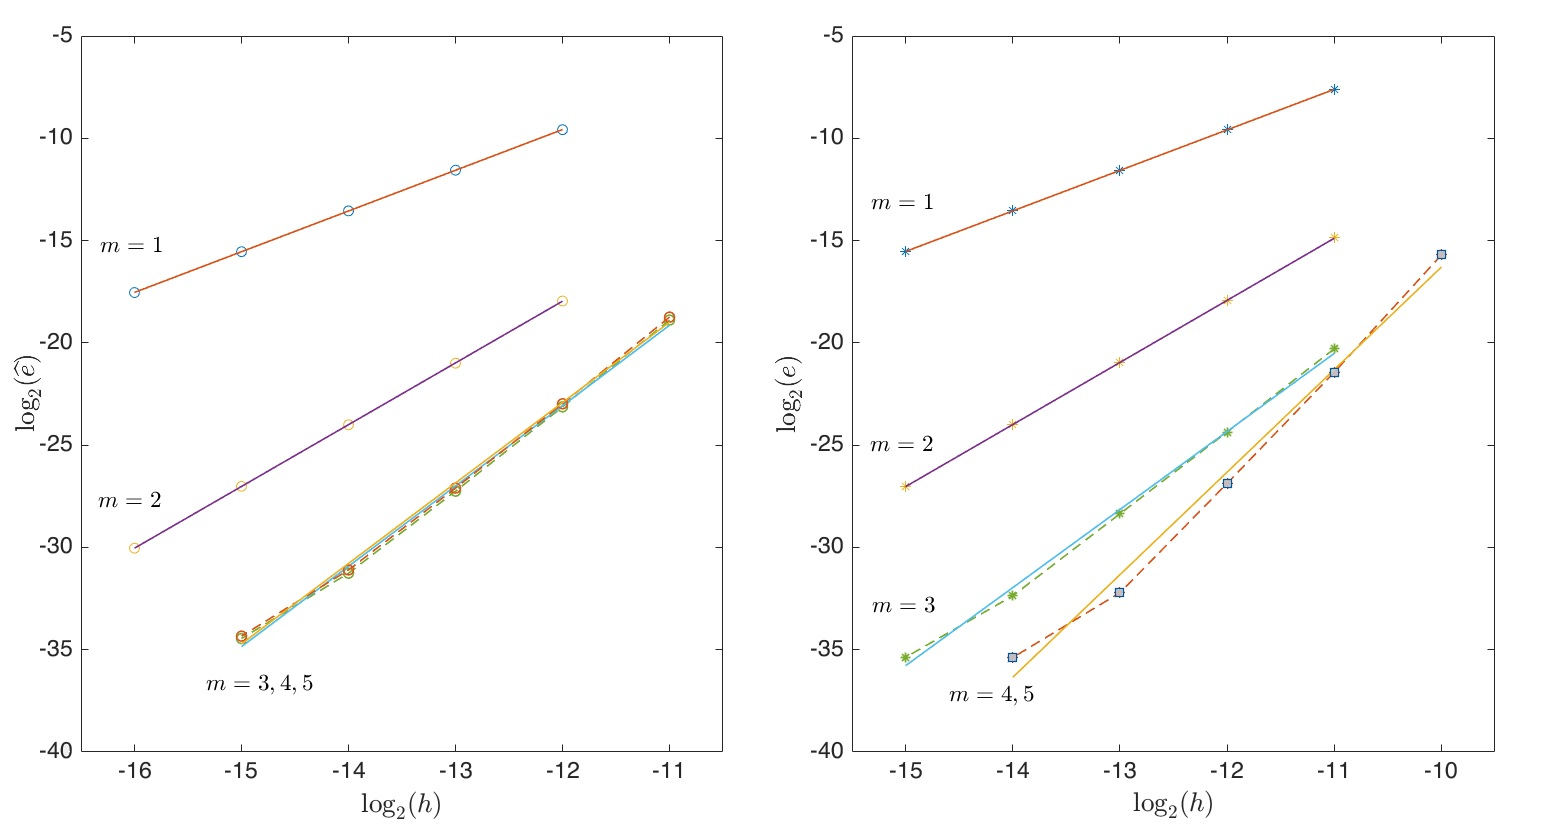
\includegraphics[scale=0.45]{Graphics/lldp/m-plots.jpg}
		\caption{Gráficos log-log de los errores $\widehat{e}_i=\max_{t_n\in(t)_{h_i}}\nnnorm{\widehat{y}_n-x(t_n)}_\infty$ y $e_i=\max_{t_n\in(t)_{h_i}}\nnnorm{y_n-x(t_n)}_\infty$ contra $h_i$ en la integración de la ecuación del Ejemplo \ref{ex:Brus} con las fórmulas (\ref{LLDPK scheme}), $\pf=6$, $\mf=1,2,3,4,5$ y $h_i=2^{-i}$, $i=10,11,12,13,14,15,16$.}
		\label{fig:num-exp-lldp-fix-step:Fig3}
	\end{center}
\end{figure}

\begin{table}[htb]
	\centering
	\caption{
        Orden de convergencia $r$ de las fórmulas (\ref{LLDPK scheme}) y su estimado  $\widetilde{r}$ para diferentes valores de $\mf$, el intervalo de $90\%$ de confianza $[\widetilde{r}-\varDelta,\widetilde{r}+\varDelta]$ y el coeficiente de determinación $R^2$ de la línea ajustada en la Figura \ref{fig:num-exp-lldp-fix-step:Fig3}.}
		\begin{tabular}{ c  c c c c  c  c c c c}
			\hline
			& \multicolumn{4}{c}{$\widehat{y}$} & & \multicolumn{4}{c}{$y$} \\
			\cline{2-5} \cline{7-10}
			$\mf$ & $r$ & $\widetilde{r}$ & $\pm\varDelta$ & $R^2$ & & $r$ & $\widetilde{r}$ & $\pm\varDelta$ & $R^2$ \\
			\hline
			1 & 2 & 1.99 & 0.01 & 0.99 & & 2 & 1.98 & 0.01 & 0.99 \\
			2 & 3 & 3.02 & 0.01 & 0.99 & & 3 & 3.04 & 0.01 & 0.99 \\
			3 & 4 & 3.93 & 0.20 & 0.99 & & 4 & 3.82 & 0.20 & 0.99 \\
			4 & 4 & 3.93 & 0.19 & 0.99 & & 5 & 5.02 & 0.45 & 0.99 \\
			5 & 4 & 3.93 & 0.19 & 0.99 & & 5 & 5.01 & 0.47 & 0.99 \\
			\hline
		\end{tabular}
	\label{tab:num-exp-lldp-fix-step:morders}
\end{table}

\begin{figure}[htb]
	\begin{center}
		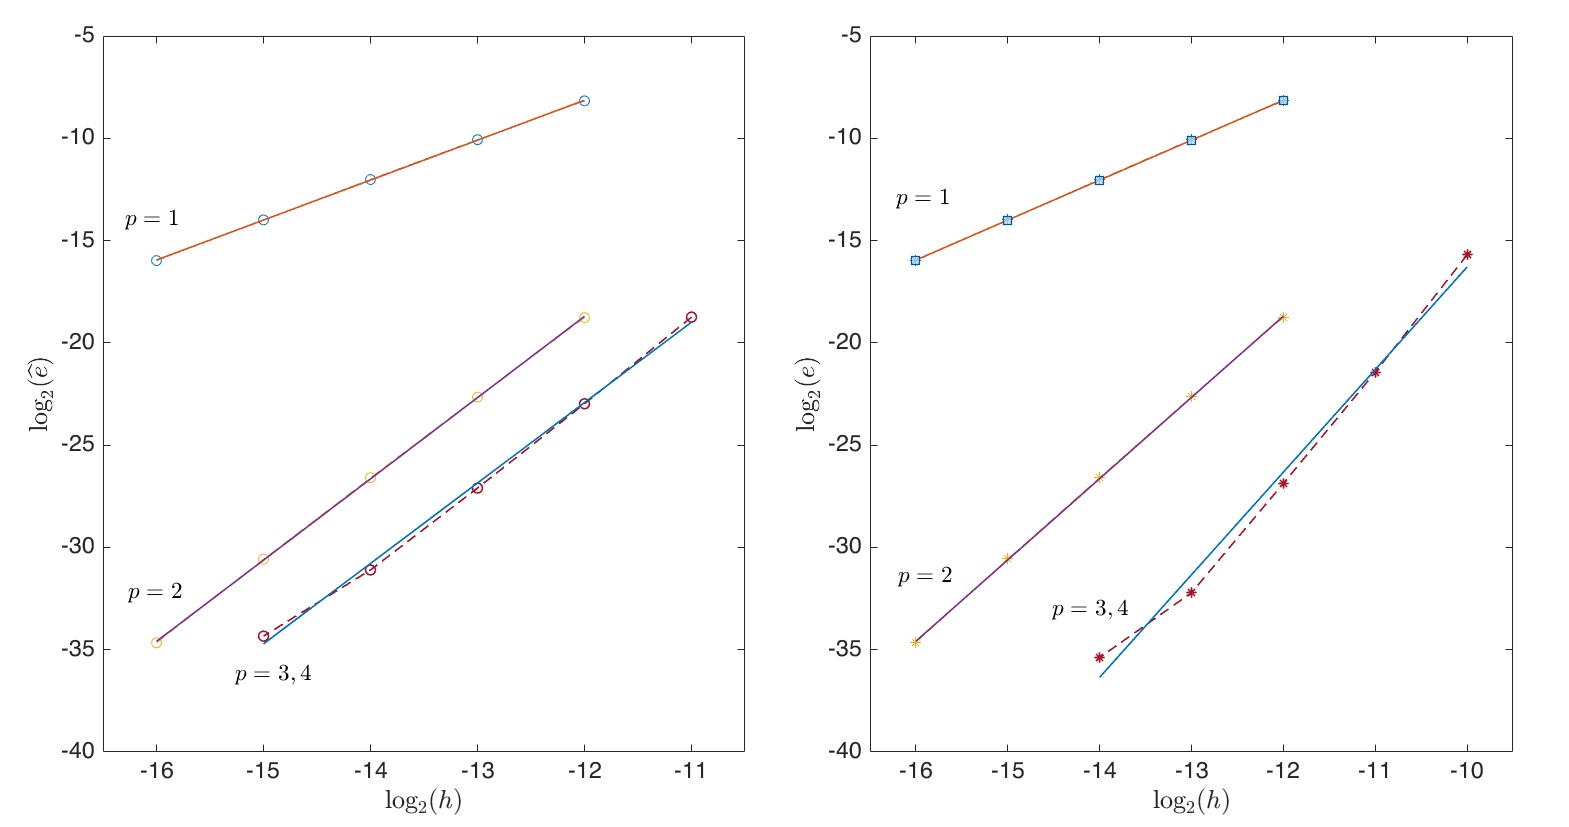
\includegraphics[scale=0.45]{Graphics/lldp/p-plots.jpg}
		\caption{Gráficos log-log de los errores $\widehat{e}_i=\max_{t_n\in(t)_{h_i}}\nnnorm{\widehat{y}_n-x(t_n)}_\infty$ y $e_i=\max_{t_n\in(t)_{h_i}}\nnnorm{y_n-x(t_n)}_\infty$ contra $h_i$ en al integración de la ecuación del Ejemplo \ref{ex:Brus} con las fórmulas (\ref{LLDPK scheme}), $\pf=1,2,3,4$, $\mf=11$ y $h_i=2^{-i}$, $i=10,11,12,13,14,15,16$.}
		\label{fig:num-exp-lldp-fix-step:Fig2}
	\end{center}
\end{figure}


\begin{table}[htb]
	\centering
	\caption{
		Orden de convergencia $r$ de las fórmulas (\ref{LLDPK scheme}) y su estimado  $\widetilde{r}$ para diferentes valores de $\pf$, el intervalo de $90\%$ de confianza $[\widetilde{r}-\varDelta,\widetilde{r}+\varDelta]$ y el coeficiente de determinación $R^2$ de la línea ajustada en la Figura \ref{fig:num-exp-lldp-fix-step:Fig2}.}
		\begin{tabular}{ c  c c c c  c  c c c c}
			\hline
			& \multicolumn{4}{c}{$\widehat{y}$} & & \multicolumn{4}{c}{$y$} \\
			\cline{2-5} \cline{7-10}
			$\pf+\pf$ & $r$ & $\widetilde{r}$ & $\pm\varDelta$ & $R^2$ & & $r$ & $\widetilde{r}$ & $\pm\varDelta$ & $R^2$ \\
			\hline
			2 & 2 & 1.95 & 0.02 & 0.99 & & 2 & 1.95 & 0.02 & 0.99 \\
			4 & 4 & 3.97 & 0.04 & 0.99 & & 4 & 3.97 & 0.04 & 0.99 \\
			6 & 4 & 3.93 & 0.19 & 0.99 & & 5 & 5.01 & 0.48 & 0.99 \\
			8 & 4 & 3.93 & 0.19 & 0.99 & & 5 & 5.01 & 0.47 & 0.99 \\
			\hline
		\end{tabular}
	\label{tab:num-exp-lldp-fix-step:porders}
\end{table}

\begin{figure}[htb]
	\begin{center}
		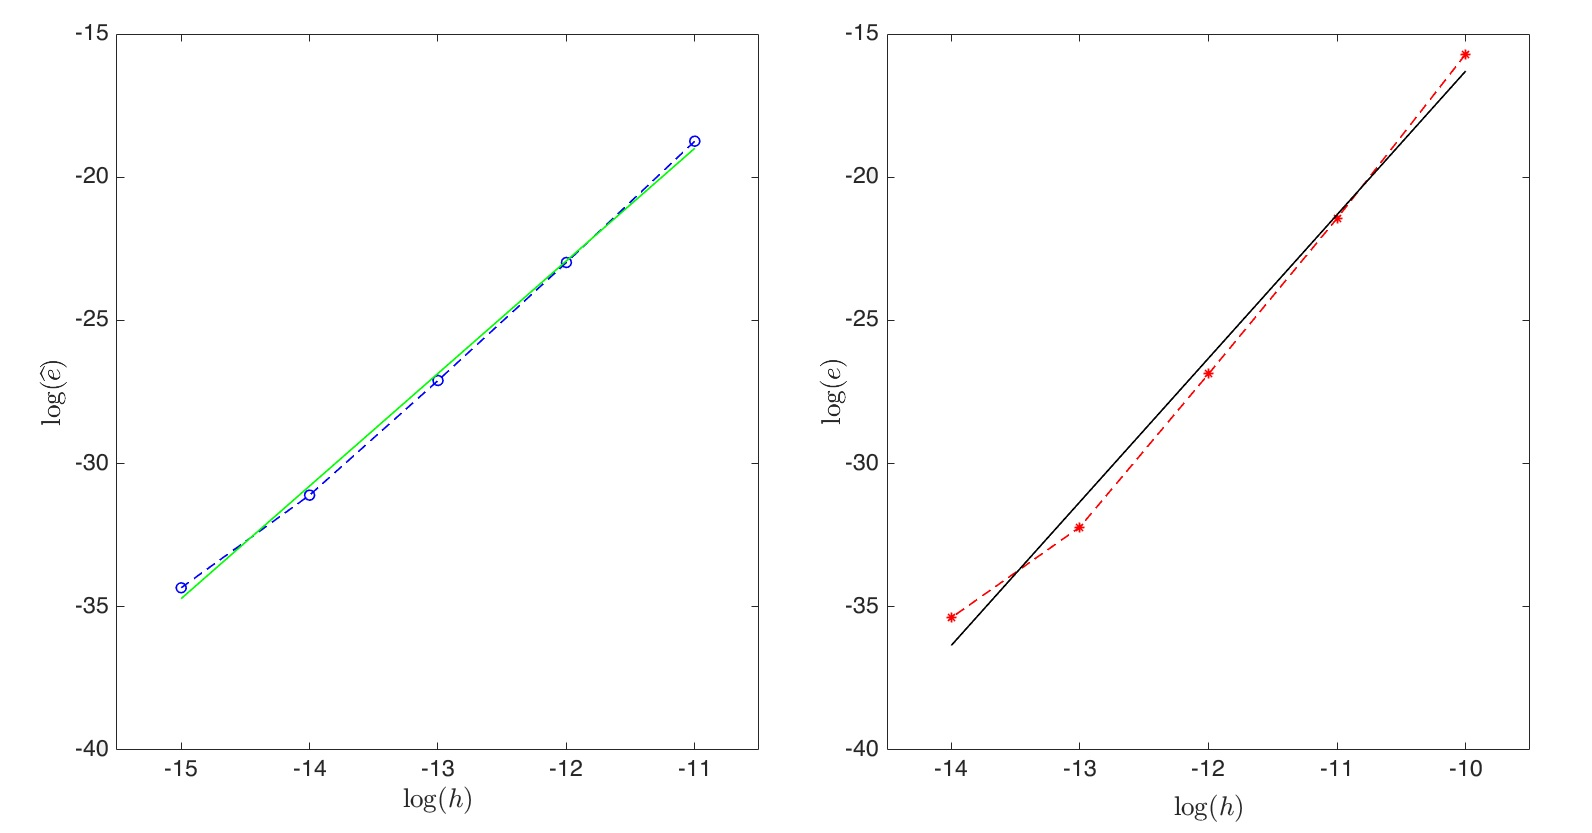
\includegraphics[scale=0.45]{Graphics/lldp/LLDP-plots.jpg}
		\caption{ Gráficos log-log de los errores $\widehat{e}_i=\max_{t_n\in(t)_{h_i}}\nnnorm{\widehat{y}_n-x(t_n)}_\infty$ y $e_i=\max_{t_n\in(t)_{h_i}}\nnnorm{y_n-x(t_n)}_\infty$ contra $h_i$ en al integración de la ecuación del Ejemplo \ref{ex:Brus} con las fórmulas (\ref{LLDPK scheme}), $\pf=6$, $\mf=11$ y $h_i=2^{-i}$, $i=10,11,12,13,14,15$.}
		\label{fig:num-exp-lldp-fix-step:Fig4}
	\end{center}
\end{figure}

\subsubsection{Simulaciones comparativas}
\importantcodes{LLDP4: esquema Runge-Kutta Localmente Linealizado de Dromand y Prince de orden 4 y paso fijo descrito en Algoritmo \ref{alg:integratorfix}}
\importantcodes{LLDP5: esquema Runge-Kutta Localmente Linealizado de Dromand y Prince de orden 5 y paso fijo descrito en Algoritmo \ref{alg:integratorfix}}
\importantcodes{expms4: esquema exponencial de Adams de orden 4 y paso fijo}
\importantcodes{expms5: esquema exponencial de Adams de orden 5 y paso fijo}
Para este segundo conjunto de simulaciones, se consideraran los esquemas numéricos definidos en el Algoritmo \ref{alg:integratorfix} para las fórmulas (\ref{LLDPK scheme}) de orden $4$ y $5$ que se implementan, respectivamente, en los códigos \emph{LLDP4} y \emph{LLDP5}. Además, se considerará, el código \textquoteleft expms\textquoteright~con orden $4$ y $5$ disponible en \cite{jansing2011expode}, que proporciona una implementación de tamaño de paso fijo de orden $4$ y $5$ para el método exponencial de Adams~\cite{hochbruck2011exponential}. Los códigos de estos dos equemas exponeciales se denotarán como \emph{expms4} y \emph{expms5}, respectivamente.

Para preservar el orden de convergencia de las fórmulas (\ref{LLDPK scheme}), se utilizaran los valores $m_{min}=3$ y $m_{min}=4$ en los códigos \emph{LLDP4} y \emph{LLDP5}, respectivamente, como lo indica el Teorema \ref{theorem:lldp-convergence}. Por el contrario, los códigos \emph{expms4} y \emph{expms5} no restringen los valores de $m_{min}$. Las tolerancias $RTol$ relativa y $ATol$ absoluta para calcular las aproximaciones de Krylov a $u_j$ se establecieron en $10^{-9}$ y $10^{-12}$, respectivamente.

Los resultados en la integración de cada ecuación de prueba obtenidos con los códigos antes mencionados se resumen en una tabla. La precisión de cada código se mide por el error relativo
\begin{equation}\label{num-exp-lldp-fix-step:ER}
	RError = \max_{i=1,\ldots,d} \;\ \max_{t_n\in(t)_h}  \;\ \left\lvert\frac{x^{[i]}(t_j)-y^{[i]}(t_j)}{\maxx{x^{[i]}(t_j),\epsilon_{mach}}}\right\rvert
\end{equation}
entre la \textquotedblleft solución exacta\textquotedblright~$x$ de la ecuación de prueba y la solución aproximada $y$ de cada código, donde $\epsilon_{mach}$ denota el épsilon de la máquina. Siguiendo \cite{tokman2006efficient}, la \textquotedblleft solución exacta\textquotedblright~de las ecuaciones de prueba se estima mediante el código Matlab \textit{ode15s} con tolerancias $RTol=10^{-12}$ y $ATol=10^{-14}$. En cada tabla, la columna \textit{RTime} presenta el tiempo computacional total relativo de cada código con respecto al código \emph{expms4} en la integración de cada ejemplo. Esta relación de tiempo general funciona como un indicador simple para comparar el costo computacional total de cada código. Las tablas también muestran el número de pasos de integración $Steps$, el número de evaluaciones de campos vectoriales \textit{f-Eval}, el número de evaluaciones de la matriz Jacobianas \textit{J-Eval}, el número de aproximaciones del subespacio de Krylov \textit{K-subspace}, la dimensión mínima $\mf_{min}$, la dimensión máxima $\mf_{max}$ y la dimensión total $\mf_{total}$ de los subespacios de Krylov utilizados por cada código en la integración de las ecuaciones de prueba con tamaño de paso $h$, donde $m_{total}$ es la suma acumulada de la dimensión de los subespacios de Krylov utilizada en cada paso de integración. En las tablas, $d$ especifica el número de ecuaciones de cada ejemplo de prueba.

Las Tablas \ref{tab:num-exp-lldp-fix-step:cpna} - \ref{tab:num-exp-lldp-fix-step:brna} presentan los resultados de la integración de las ecuaciones de prueba de los Ejemplos \ref{ex:cusp}-\ref{ex:Brus}, mostrando que, con tamaño de paso fijo y dimensión variable de Krylov, los códigos \emph{LLDP4} y \emph{LLDP5} son más precisos que los códigos \emph{expms4} y \emph{expms5}, con un costo computacional similar o menor. Los códigos \emph{LLDP} son más rápidos porque requieren el cálculo de solo un subespacio de Krylov por paso de integración con dimensiones más pequeñas, mientras que los otros códigos calculan más de un subespacio de Krylov con dimensiones más altas. El código \emph{LLDP5} es más rápido que el \emph{LLDP4} porque la fórmula de orden 4 en (\ref{LLDPK scheme}) requiere de una evaluación adicional del campo vectorial $f$ en cada paso de integración. Con tamaño de paso $h = 0.0064$, el código \emph{expms5} produce desbordamiento en la precisión del punto flotante~(\textit{overflow} en inglés) en la integración de la ecuación de Burges, razón por la cual falta información en la Tabla \ref{tab:num-exp-lldp-fix-step:bgna}. Por la misma razón, falta un valor en la Tabla \ref{tab:num-exp-lldp-fix-step:brna} para el código \emph{expms5} con un tamaño de paso $h = 0.0008$.

Además, las tablas muestran la efectividad de la estrategia propuesta para la selección de la dimensión de Krylov $\mf$ en cada paso de integración, con mínima variación entre los valores de $\mf_{min}$ y $\mf_{max}$, y así, con un valor menor de $\mf_{total}$.

\begin{table}[htb]
	\caption{Desempeño de los códigos de paso fijo \emph{expms4}, \emph{expms5}, \emph{LLDP4} y \emph{LLDP5} en la integración de la ecuación CUSP con $M=32$, $d=96$.}
	\centering
	\begin{adjustbox}{width=0.95\columnwidth,center}
		\begin{tabular}{lccccccccc}
			\hline
			& RTime & RError & Steps & f-Eval & J-Eval & K-subspace & $\mf_{total}$ & $\mf_{min}$ & $\mf_{max}$ \\
			\hline
			h = 0.000001 &  &  &  &  &  &  &  &  &  \\
			expms4 & 1.0000 & 8.4400e-01 & 100 & 204 & 100 & 298 & 1131 & 2 & 6  \\
			expms5 & 1.1863 & 6.1635e-01 & 100 & 209 & 100 & 397 & 1336 & 2 & 6  \\
			LLDP4 & 0.1013 & 3.8321e-08 & 100 & 700 & 100 & 100 & 400 & 4 & 4  \\
			LLDP5 & 0.0863 & 1.0889e-09 & 100 & 600 & 100 & 100 & 400 & 4 & 4  \\
			\hline
			h = 0.000005 &  &  &  &  &  &  &  &  &  \\
			expms4 & 1.0000 & 9.7513e-01 & 20 & 44 & 20 & 58 & 381 & 4 & 11  \\
			expms5 & 1.0480 & 1.0766e+00 & 20 & 49 & 20 & 77 & 593 & 4 & 20  \\
			LLDP4 & 0.0354 & 4.5302e-06 & 20 & 140 & 20 & 20 & 130 & 6 & 7  \\
			LLDP5 & 0.0338 & 2.0199e-07 & 20 & 120 & 20 & 20 & 130 & 6 & 7  \\
			\hline
			h = 0.000010 &  &  &  &  &  &  &  &  &  \\
			expms4 & 1.0000 & 1.7607e+00 & 10 & 24 & 10 & 28 & 378 & 6 & 36  \\
			expms5 & 1.1111 & 3.5472e+02 & 10 & 29 & 10 & 37 & 586 & 6 & 36  \\
			LLDP4 & 0.0228 & 4.4774e-05 & 10 & 70 & 10 & 10 & 83 & 7 & 10  \\
			LLDP5 & 0.0214 & 1.3267e-05 & 10 & 60 & 10 & 10 & 83 & 7 & 10  \\
			\hline
		\end{tabular}
	\end{adjustbox}
	\label{tab:num-exp-lldp-fix-step:cpna}
\end{table}



\begin{table}[htb]
	\caption{Desempeño de los códigos de paso fijo \emph{expms4}, \emph{expms5}, \emph{LLDP4} y \emph{LLDP5} en la integración de la ecuación Burgers con $M=500$, $d=500$.}
	\centering
	\begin{adjustbox}{width=0.95\columnwidth,center}
	\begin{tabular}{lccccccccc}
		\hline
		& RTime & RError & Steps & f-Eval & J-Eval & K-subspace & $\mf_{total}$ & $\mf_{min}$ & $\mf_{max}$ \\
		\hline
		h = 0.001600 &  &  &  &  &  &  &  &  &  \\
		expms4 & 1.0000 & 2.0411e-03 & 313 & 630 & 313 & 937 & 5984 & 2 & 11  \\
		expms5 & 1.3115 & 6.2805e-04 & 313 & 635 & 313 & 1249 & 7744 & 2 & 11  \\
		LLDP4 & 0.1109 & 3.7647e-06 & 313 & 2191 & 313 & 313 & 2174 & 4 & 8  \\
		LLDP5 & 0.1081 & 6.8065e-07 & 313 & 1878 & 313 & 313 & 2174 & 4 & 8  \\
		\hline
		h = 0.003200 &  &  &  &  &  &  &  &  &  \\
		expms4 & 1.0000 & 2.0005e-02 & 157 & 318 & 157 & 469 & 5802 & 3 & 46  \\
		expms5 & 1.2350 & 1.1603e-02 & 157 & 323 & 157 & 625 & 7747 & 3 & 57  \\
		LLDP4 & 0.0719 & 7.8449e-05 & 157 & 1099 & 157 & 157 & 1425 & 6 & 10  \\
		LLDP5 & 0.0719 & 4.5654e-05 & 157 & 942 & 157 & 157 & 1425 & 6 & 10  \\
		\hline
		h = 0.006400 &  &  &  &  &  &  &  &  &  \\
		expms4 & 1.0000 & 5.7742e-01 & 79 & 162 & 79 & 235 & 6267 & 6 & 100  \\
		expms5 & - & - & - & - & - & - &- & - & -\\
		LLDP4 & 0.0281 & 2.3688e-03 & 79 & 553 & 79 & 79 & 954 & 8 & 14  \\
		LLDP5 & 0.0278 & 3.6646e-03 & 79 & 474 & 79 & 79 & 964 & 8 & 15  \\
		\hline
	\end{tabular}
\end{adjustbox}
	\label{tab:num-exp-lldp-fix-step:bgna}
\end{table}


\begin{table}[htb]
	\caption{Desempeño de los códigos de paso fijo \emph{expms4}, \emph{expms5}, \emph{LLDP4} y \emph{LLDP5} en la integración de la ecuación Brusselator2D con $M=50$, $d=5000$.}
	\centering
	\begin{adjustbox}{width=0.95\columnwidth,center}
	\begin{tabular}{lccccccccc}
		\hline
		& RTime & RError & Steps & f-Eval & J-Eval & K-subspace & $\mf_{total}$ & $\mf_{min}$ & $\mf_{max}$ \\
		\hline
		h = 0.000313 &  &  &  &  &  &  &  &  &  \\
		expms4 & 1.0000 & 2.7423e-09 & 320 & 644 & 320 & 958 & 1702 & 1 & 6  \\
		expms5 & 1.3830 & 2.6788e-09 & 320 & 649 & 320 & 1277 & 2023 & 1 & 6  \\
		LLDP4 & 0.7161 & 1.9118e-10 & 320 & 2240 & 320 & 320 & 960 & 3 & 3  \\
		LLDP5 & 0.7158 & 9.6701e-12 & 320 & 1920 & 320 & 320 & 1280 & 4 & 4  \\
		\hline
		h = 0.006250 &  &  &  &  &  &  &  &  &  \\
		expms4 & 1.0000 & 7.7678e-06 & 16 & 36 & 16 & 46 & 231 & 3 & 11  \\
		expms5 & 1.1151 & 3.5951e-06 & 16 & 41 & 16 & 61 & 283 & 2 & 11  \\
		LLDP4 & 0.2909 & 1.7453e-08 & 16 & 112 & 16 & 16 & 115 & 6 & 9  \\
		LLDP5 & 0.2592 & 4.8969e-09 & 16 & 96 & 16 & 16 & 115 & 6 & 9  \\
		\hline
		h = 0.012500 &  &  &  &  &  &  &  &  &  \\
		expms4 & 1.0000 & 5.4570e-05 & 8 & 20 & 8 & 22 & 163 & 4 & 15  \\
		expms5 & 1.0989 & 3.1705e-05 & 8 & 25 & 8 & 29 & 213 & 4 & 15  \\
		LLDP4 & 0.1990 & 1.6384e-07 & 8 & 56 & 8 & 8 & 74 & 8 & 11  \\
		LLDP5 & 0.1783 & 9.7264e-08 & 8 & 48 & 8 & 8 & 74 & 8 & 11  \\
		\hline
	\end{tabular}
\end{adjustbox}
	\label{tab:num-exp-lldp-fix-step:br2dna}
\end{table}

\begin{table}[htb]
	\caption{Desempeño de los códigos de paso fijo \emph{expms4}, \emph{expms5}, \emph{LLDP4} y \emph{LLDP5} en la integración de la ecuación Brusselator con $M=100$, $d=200$.}
	\centering
	\begin{adjustbox}{width=0.95\columnwidth,center}
	\begin{tabular}{lccccccccc}
		\hline
		& RTime & RError & Steps & f-Eval & J-Eval & K-subspace & $\mf_{total}$ & $\mf_{min}$ & $\mf_{max}$ \\
		\hline
		h = 0.000200 &  &  &  &  &  &  &  &  &  \\
		expms4 & 1.0000 & 1.8209e-01 & 5000 & 10004 & 5000 & 14998 & 37224 & 1 & 6  \\
		expms5 & 1.2761 & 2.2454e-01 & 5000 & 10009 & 5000 & 19997 & 42325 & 1 & 6  \\
		LLDP4 & 0.1876 & 4.2112e-08 & 5000 & 35000 & 5000 & 5000 & 15491 & 3 & 6  \\
		LLDP5 & 0.1839 & 2.3705e-09 & 5000 & 30000 & 5000 & 5000 & 20004 & 4 & 6  \\
		\hline
		h = 0.000400 &  &  &  &  &  &  &  &  &  \\
		expms4 & 1.0000 & 3.6729e-01 & 2500 & 5004 & 2500 & 7498 & 23266 & 1 & 8  \\
		expms5 & 1.2349 & 4.4819e-01 & 2500 & 5009 & 2500 & 9997 & 25921 & 1 & 8  \\
		LLDP4 & 0.1915 & 7.8097e-07 & 2500 & 17500 & 2500 & 2500 & 10068 & 4 & 6  \\
		LLDP5 & 0.1621 & 9.7577e-08 & 2500 & 15000 & 2500 & 2500 & 10068 & 4 & 6  \\
		\hline
		h = 0.000800 &  &  &  &  &  &  &  &  &  \\
		expms4 & 1.0000 & 7.2534e-01 & 1250 & 2504 & 1250 & 3748 & 15258 & 2 & 8  \\
		expms5 & - & - & - & - & - & - &- & - & -\\
		LLDP4 & 0.1873 & 1.5639e-05 & 1250 & 8750 & 1250 & 1250 & 7517 & 6 & 8  \\
		LLDP5 & 0.1805 & 4.6983e-06 & 1250 & 7500 & 1250 & 1250 & 7517 & 6 & 8  \\
		\hline
	\end{tabular}
\end{adjustbox}
	\label{tab:num-exp-lldp-fix-step:brna}
\end{table}

\section{Esquemas adaptativos con tamaño de paso variable}
Para escribir un código que determine automáticamente el tamaños de paso lo suficientemente pequeños para obtener la precisión adecuada y lo suficientemente grandes para evitar trabajo computacional innecesario, es necesaria una estrategia adaptativa adecuada. Como se mostró en \cite{Jimenez14AMC}, el control del tamaño de paso automático de las fórmulas embebidas originales de Dormand y Prince se adapta bien a las fórmulas embebidas (\ref{LLDPK scheme}) para PVI pequeños. Es fácil notar que con ciertas modificaciones relacionadas con la aproximación Krylov-Padé (\ref{eq:kp_aprox}), esta estrategia para la selección del tamaño del paso parece adecuada para las fórmulas embebidas (\ref{LLDPK scheme}) para PVI de dimensiones no pequeñas. A continuación, se describirá la estrategia adaptativa para las fórmulas embebidas (\ref{LLDPK scheme}).

\subsection{Estimación del tamaño de paso}\label{secc:stepsizes}
Se denotará por $h_{max}$ y $h_{min}$ los tamaños de paso máximos y mínimos permisibles. La estimación de los tamaños de paso se calcula mediante las mismas expresiones utilizadas para las fórmulas originales de Dormand y Prince en el código de Matlab \textit{ode45} \cite{shampine1997matlab} y para las fórmulas embebidas en \cite{Jimenez14AMC}. Para el tamaño de paso inicial $h_0$, tenemos la estimación
\begin{equation}
    h_0 = \minn{ h_{max}, \maxx{ h_{min} ,\Delta} }, \label{hcero}
\end{equation}
donde
\begin{equation*}
    \Delta = \begin{cases}
        \frac{1}{r_h} & \text{si} \; h_{max}\cdot r_h>1\\
        h_{max} & \text{en otro casos}
        \end{cases}
\end{equation*}
con
\begin{equation*}
     r_h = \frac{1\mathord{.}25}{RTol^{1/5}}\max_{i=1\ldots d}\left\{\frac{ \left\lvert f^{[i]}(t_0,y_0) \right\rvert }
    {\maxx{\left\lvert y^{[i]}_0 \right\rvert ,\frac{ATol}{RTol}}}\right\}.
\end{equation*}

Todos los demás tamaños de paso nuevos $h_{new}$ se estiman mediante la expresión
\begin{equation}
    h_{new} = \minn{h_{max},\maxx{h_{min},\Delta}}, \label{hnewcalc}
\end{equation}
donde
\begin{equation*}
    \Delta = \begin{cases}
        h_n/\rho & \text{si } \varepsilon_y\leq RTol \text{ y } \rho>0\mathord{.}2\\
        5\cdot h_n & \text{si } \varepsilon_y\leq RTol \text{ y } \rho\leq 0\mathord{.}2\\
        \maxx{0\mathord{.}1,1/\rho}\cdot h_n & \text{si } \varepsilon_y > RTol \text{ y } fail=false\\
        0\mathord{.}5\cdot h_n & \text{si } \varepsilon_y > RTol \text{ y } fail=true
        \end{cases},
\end{equation*}
siendo
\begin{equation}\label{epsilon_y}
	\varepsilon_y =  \max_{i=1\ldots d}\left\{ \frac{\left\lvert y^{[i]}_{n+1}-\hat{y}^{[i]}_{n+1} \right\rvert}
	{\maxx{\left\lvert y^{[i]}_{n+1}  \right\rvert,\left\lvert y^{[i]}_{n}\right\rvert,\frac{ATol}{RTol}}} \right\}
\end{equation}
la medida del error relativo entre las fórmulas integradas $y$ y $\hat{y}$ definidas en (\ref{LLDPK scheme}), y $fail$ indica que se rechazó un tamaño de paso anterior en $t_n$.

\subsection{Control del tamaño de paso}\label{secc:hcontrol}
Como en \cite{Jimenez14AMC}, para obtener una tolerancia deseada y evitar el desbordamiento en el cálculo de la matriz exponencial $e^{\frac{1}{90}h_n\overline{H}}$ a través de la aproximación $(\pf,\pf)$-Padé con escalamiento y potenciación, el valor de $\left\Vert \frac{1}{90}h_n\overline{H} \right\Vert_\infty$ debe ser controlado. Debido a los errores de redondeo, si
\begin{equation}
	\left\Vert \frac{1}{90}h_n\overline{H} \right\Vert_\infty \ge 600\,,  \label{eq:H-bound-1} 
\end{equation}
 la aproximación de Padé a $e^{\frac{1 }{90}h_n\overline{H}}$ carece de precisión. Dado que $H_\mf$ en (\ref{hhat}) es la matriz de Hessenberg correspondiente a $\mathcal{K}_\mf(f_x,f)$, el Lema \ref{H-bound} implica que 
 \begin{equation}
 	|| \overline{H} ||_\infty \leq 1 + || f_x ||_\infty\,.  \label{eq:H-bound-2}
 \end{equation}
 Las desigualdades (\ref{eq:H-bound-1}) y (\ref{eq:H-bound-2}) implican que si $h_n + \left\lVert h_nf_x \right\rVert_\infty \leq 54000$, entonces la aproximación $(\pf,\pf)$-Padé de $e^{\frac{1}{90}h_n \overline{H}}$ conserva la precisión establecida en la Tabla \ref{table:padep} para el valor dado de $\pf$. Así, en la práctica, si $h_n + \left\lVert h_nf_x \right\rVert_\infty \ge 54000$, el valor de $h_n$ se recalcula como $h_n=\frac{54000}{1+\left\lVert f_x \right\rVert_\infty}$.

Aquí hay que tener en cuenta que en el caso de que se modifique el valor del tamaño de paso $h_{n}$, la evaluación de $f$ y $f_x$ en $y_n$ realizada para calcular $\overline{H}$ es reutilizada. Por lo tanto, este reemplazo de tamaño de paso no se considera como un paso fallido ``típico'' .

\subsection{Reutilización de la matriz Jacobiana}\label{secc:jaccontrol}
Ciertamente, para PVI de grandes dimensiones almacenar y evaluar la matriz Jacobiana densa en cada paso de integración es una tarea computacionalmente exigente. Sin embargo, por lo general, la matriz Jacobiana de los grandes sistemas de PVI resultantes de la discretización espacial de las EDP tiene una estructura esparcida. En esta situación, en la práctica, es posible almacenar y reutilizar esas matrices. Para determinar cuándo el Jacobiano evaluado en un paso de integración se puede reutilizar en pasos de integración consecutivos, se necesita establecer una medida de disimilitud entre el Jacobiano $J=f_x(y_n)$ en el paso de integración actual $n$ con el Jacobiano $J_{old}= f_x(y_{i})$ en un paso de integración anterior $i<n$. Una de tales medidas de disimilitud se puede definir en términos de
\begin{equation*}
    \Delta \mathcal{J} = J\cdot f(y_n) - J_{old}\cdot f(y_n),
\end{equation*}
o por la expresión relativa
\begin{equation}\label{jerror}
    \varepsilon_J = \max_{l=1\ldots d}\frac{\nnorm{\Delta \mathcal{J}^{[l]}}}
    {\maxx{\nnorm{ \left(J_{old}\cdot f_{old}\right)^{[l]} } ,\frac{ATol}{RTol}}},
\end{equation}
donde $f_{old}=f(y_i)$.

Dado que en la expresión ~(\ref{jerror}) se supone que el Jacobiano $J$ en $y_n$ no se evalúa, el término $J\cdot f(y_n)$ es
aproximado por el cociente diferencial hacia atrás
\begin{equation}\label{backapprox}
    J\cdot f(y_n) \approx \frac{f(y_n) -
        f\left(y_n-\delta f(y_n)\right)}{\delta}
\end{equation}
para un $\delta>0$ lo suficientemente pequeño. Pero, en esta aproximación se requiere la evaluación de $f$ en un punto medio. Para evitar esto, se puede usar la aproximación convexa
\begin{equation}\label{aproxaprox}
    f\left(y_n-\delta f(y_n)\right) \approx
    (1-\delta) f(y_n)+ \delta \; \mathtt{K},
\end{equation}
donde $K = \kt_{6} + f(y_{n-1}) + J_{old}\widetilde{u}_{6} $ y
\[ \kt_6 = f\left( y_{n-1}+\widetilde{u}_6+h_{n-1} \sum_{i=1}^{5}a_{6,i}\kt_i \right) - f(y_{n-1}) - J_{old}\widetilde{u}_6 \]
es el estado $6$ del esquema~(\ref{LLDPK scheme}) ya calculado en el paso anterior $n-1$.

Es importante notar que el campo vectorial $f$ en el punto actual $y_n$ tiene el mayor peso en la aproximación porque $\delta$
es pequeño. Sustituyendo~(\ref{backapprox})-(\ref{aproxaprox}) en (\ref{jerror}) se obtiene que
\begin{equation}\label{jerroraprox}
    \varepsilon_J = \max_{l=1\ldots d}\frac{\nnorm{f^{[l]}(y_n) - \mathtt{K}^{[l]} - (J_{old}\cdot f(y_n))^{[l]}}}
    {\maxx{\nnorm{ \left(J_{old}\cdot f_{old}\right)^{[l]} } ,\frac{ATol}{RTol}}}.
\end{equation}

Con esta medida relativa de disimilitud, el Jacobiano se evalúa en el punto $y_n$ solo si $\gamma_J \cdot \varepsilon_J \geq 1$, donde $\gamma_J=\frac{1}{8}$ es un factor de seguridad. Este procedimiento para la reutilización de la matriz Jacobiana se resume en las líneas 3 a 12 del Algoritmo \ref{alg:jaccontrol} y se utiliza siempre que el tamaño de paso $h_n$ en el paso de integración $n$ no haya sido rechazado previamente. De lo contrario, el Jacobiano siempre se actualiza como se indica en las líneas 15 a 20 del mismo Algoritmo.

{\SetAlgoNoLine
\begin{algorithm}[htb]
	\caption{Algoritmo de control para la reutilización de la matriz Jacobiana}
	\label{alg:jaccontrol}
	\KwIn{$n$,$y_n$,$fail,J,J_{old},f_{old},freshJ$}
	\KwOut{$J,J_{old},f_{old},freshJ$}
	\eIf{$fail=false$}{
		\If{$n>0$}{
			Calcular la medida relativa de disimilitud $\varepsilon_J$ mediante (\ref{jerroraprox})\\
			\eIf{$\gamma_J\cdot\varepsilon_J \geq 1$}{
				$J=f_x(y_n)$ \\
				$J_{old} = J$ \\
				$f_{old} = f(y_n)$ \\
				$freshJ=true$ \\
			}
			{
				$J=J_{old}$ \\
				$freshJ=false$ \\
			}
		}
	}
	{
		\If{$freshJ=false$}{
			$J=f_x(y_n)$ \\
			$J_{old} = J$ \\
			$f_{old} = f(y_n)$ \\
			$freshJ=true$ \\
		}
	}
\end{algorithm}
}

\subsection{Control del \textit{Breakdown}}\label{sec:brcontrol}
El \emph{breakdown} en el Algoritmo de Arnoldi~\ref{alg:Arnoldi}, línea $10$, puede ocurrir por la pérdida de ortogonalidad al generar los vectores base como consecuencia de la acumulación de errores de redondeo. Por esta razón, el Algoritmo~\ref{alg:Arnoldi} tiene una parada anticipada y el último vector en la base es inservible. Cuando ocurre \emph{breakdown} tenemos dos situaciones: 1) $\varepsilon_{K}/\gamma_K< 1$, o 2) $\varepsilon_{K}/\gamma_K \geq 1$ donde $\varepsilon_{K}$ es el error relativo (\ref{errrel}) y $\gamma_K$ su factor de seguridad.

En el caso de que $\varepsilon_{K}/\gamma_K< 1$, se acepta la aproximación de Krylov. De lo contrario, la aproximación de Krylov-Padé no satisface los requisitos de tolerancia y se calcula un nuevo valor de $h_n$. Con $h_{old}=h_n$, el nuevo valor del tamaño del paso se calcula como $h_n=\maxx{h_{min},0.9\cdot h_{old}}$. De esta forma, se debe calcular también un nuevo valor del orden de Padé $\pf$ y de la medida de error $\varepsilon_{K}$.

\subsection{Aproximación Krylov-Padé adaptativa}\label{secc:krylov-Pade}
Con una combinación adecuada de los procedimientos de las Secciones \ref{sec:selkrydim} y \ref{sec:pade-order} para la estimación óptima de la dimensión de Krylov $\mf$ y el orden de Padé $\pf$, el Algoritmo \ref{alg:errcontrol} presenta el esquema adaptativo de la aproximación de Krylov-Padé para $u_j$ en cada paso de integración.

{\SetAlgoNoLine
\begin{algorithm}[!htb]
	\caption{Algoritmo para el cálculo de las funciones $u_j$ en (\ref{LLDPK scheme}) mediante la aproximación adaptativa Krylov-Padé}
	\label{alg:errcontrol}
	\KwIn{$c_j$, $h_n$, $J$, $f$, $\mf_n$, $V_{\mf_n}$, $H_{\mf_n}$,
		$v_{\mf_{n}+1}$,  $\hf_{\mf_{n}+1,\mf_n}$, $H^*_{m_{n}}$, $breakdown$}
	\KwOut{$\widetilde{u }_j$, $h_n$, $\mf_n$, $V_{\mf_n}$,   $H_{\mf_n}$,
		$v_{\mf_{n}+1}$,  $\hf_{\mf_{n}+1,\mf_n}$, $H^*_{m_{n}}$, $\varepsilon_{K}$}
	$work=true$\\
	\While{work}{
		Selecionar el orden de Padé $\pf$ según Sección \ref{sec:pade-order} \\
		Estimar el error relativo $\varepsilon_{K}$ mediante fórmula~(\ref{errrel}) \\
		\eIf{$\varepsilon_{K}/\gamma_{K}< 1$}{
			$work=false$
		}{
			\eIf{$breakdown$ = $true$ \textbf{or} $\mf_n=\mf_{max}$}{
				$h_{new}=\maxx{h_{min},0.9\cdot h_{n}}$\\
				$h_{n}=h_{new}$\\
				\If{$h_n = h_{min}$}{work = false}
			}{
				Estimar la nueva dimensión de Krylov $\mf_{new}$ mediante fórmula
				(\ref{calcmnew}) \\
				Ejecutar Algoritmo~\ref{alg:Arnoldiexpand} para obtener matrices $H^*_{m_{new}}$ y $V_{m_{new}}$ de $\mathcal{K}_{\mf_{new}}(h_nJ,f)$, y calcular $H_{m_{new}}=H^*_{m_{new}}/h_n$\\
				Hacer $\mf_n=\mf_{new}$ y actualizar todas las variables que dependen de $\mf_n$,
			}
		}

	}
	Calcular $\widetilde{u}_j$ mediante la fórmula (\ref{eq:kp_aprox})\\
\end{algorithm}}

\subsection{Esbozo del Esquema}

Teniendo en cuenta los procedimientos de las Secciones \ref{secc:stepsizes} y \ref{secc:hcontrol} para la estimación y control del tamaño de paso $h_n$, el criterio de la Sección \ref{secc:jaccontrol} para la reutilización del Jacobiano, y la aproximación adaptativa de Krylov-Padé a $u_j$ descrita en la Sección \ref{secc:krylov-Pade}, el Algoritmo \ref{alg:integrator} presenta el esquema de la estrategia adaptativa para las fórmulas embebidas  (\ref{LLDPK scheme}) con tamaño de paso y dimensión Krylov variables. Obsérvese que, para tamaños de paso no fallidos, el Algoritmo \ref{alg:Arnoldi} es utilizado solo una vez por paso de integración. Cuando un tamaño de paso $h_n$ es rechazado, el Algoritmo \ref{alg:Arnoldi} es utilizado solo si la matriz Jacobiana no se ha actualizado en $y_n$, es decir, cuando $J \neq f_x(y_n)$.


{\SetAlgoNoLine
\begin{algorithm}[htb]
	\caption{Algoritmo del esquema de orden $5$ con tamaño de paso y dimensión de Krylov variable para las fórmulas embebidas  (\ref{LLDPK scheme})}
	\label{alg:integrator}
	\KwIn{intervalo de tiempo $[t_0, T]$, valor inicial $y_0$, tolerancia absoluta y relativa $Atol$ y $Rtol$, dimensión máxima y mínima de los subespacios de Krylov $\mf_{max}$ y $\mf_{min}$, tamaño de paso máximo $h_{max}$}
	\KwOut{$\{(t_0,y_0),\ldots,(t_n,y_n)\}$}
	$n=0$, $fail=false$, $reuse=false$, $\mf_0=\mf_{min}$, $h_{min}=16 \cdot \epsilon(t_0)$ \\
	Calcular $h_0$ mediante fórmula (\ref{hcero}) \\
	$J = f_x(y_n)$ \\
	$J_{old} = J$, $freshJ=true$ \\
	$f_{old} = f(y_n)$ \\
	\While{$t_n<T$}{
		Control de reutilización del Jacobiano mediante Algoritmo~\ref{alg:jaccontrol} \\
		Control del tamaño de paso como se especifica en la sección~\ref{secc:hcontrol} \\
		\If{$fail=false$ or $reuse=false$}{
			Ejecutar Algoritmo~\ref{alg:Arnoldi} para obtener matrices $H^*_{m_n}$ y $V_{m_n}$ de $\mathcal{K}_{\mf_n}(h_nJ,f)$, y calcular $H_{m_n}=H^*_{m_n}/h_n$ \\
		}
		Calcular $\widetilde{u}_j$ mediante Algoritmo~\ref{alg:errcontrol}\\
		Evaluar las fórmulas embebidas (\ref{LLDPK scheme}) \\
		Estimar el error (\ref{epsilon_y}) de las formulas embebidas \\
		Estimar la nueva dimensión de Krylov $\mf_{new}$ mediante fórmula (\ref{calcmnew}) \\
		Estimar le nuevo tamaño de paso $h_{new}$ mediante fórmula (\ref{hnewcalc}) \\
		\eIf{$\varepsilon_y< RTol$}{
			\If{$t_n+h_n+h_{new}>T$}{
				$h_{new}=T-(t_n+h_n)$ \\
			}
			$t_{n+1}=t_n+h_n$, $n=n+1$, $h_n=h_{new}$, $\mf_n = \mf_{new}$, $fail=false$, $reuse=false$ \\
		}
		{
			\eIf{$h_{new}>h_{min}$}
			{
				$h_n=h_{new}$, $\mf_n = \mf_{new}$, $fail = true$, $reuse=fail\,\&freshJ$
			}
			{$t_{n+1}=t_n+h_n$, $n=n+1$, $h_n=h_{new}$, $\mf_n = \mf_{new}$, $fail=false$, $reuse=false$}
		}
	$h_{min}=16 \cdot \epsilon(t_n)$
	}
\end{algorithm}}

\subsection{Experimentos numéricos}\label{section:num-exp-lldp-var-step}
\importantcodes{LLDP45: esquema adaptativo para las fórmulas embebidas Runge-Kutta de Dormand y Prince localmente linealizadas descrito en Algoritmo \ref{alg:integrator}}
En esta subsección se estudiará el desempeño del esquema adaptativo descrito en el Algoritmo \ref{alg:integrator} para las fórmulas embebidas (\ref{LLDPK scheme}). Con este propósito se implementó el código Matlab \emph{LLDP45}. Este código \emph{LLDP45} es una copia exacta del código \emph{ode45} \cite{shampine1997matlab} de Matlab18a con la excepción de las líneas del programa correspondientes a las fórmulas originales de Dormand y Prince y su error relativo, que fueron reemplazadas por las líneas 7 a 16 del Algoritmo \ref{alg:integrator} que implementan la evaluación de las fórmulas localmente linealizadas (\ref{LLDPK scheme}) con control de reutilización del Jacobiano. El código de Matlab \emph{ode45} implementa la estrategia de tamaño de paso variable descrita en la Sección \ref{secc:stepsizes} para las fórmulas embebidas de Dormand y Prince. Para preservar el orden de convergencia establecido en el Teorema \ref{theorem:lldp-convergence} para las fórmulas embebidas (\ref{LLDPK scheme}), se establece $m_{min}=4$ en el código \emph{LLDP45}.
\importantcodes{ode15s: esquema adaptativo para las fórmulas diferenciales hacia atrás de orden variable 1-5}
Los resultados del código \emph{LLDP45} en la integración de las ecuaciones de prueba de Sección \ref{section:test-eq} se compararán con los obtenidos por el código adaptativo \emph{ode15sk} con una implementación de tamaño de paso casi constante de las fórmulas diferenciales hacia atrás (BDF) hasta orden 5 y un método de subespacios de Krylov para resolver sistemas lineales de ecuaciones algebraicas. Para comparar con una implementación eficiente de estas fórmulas, este código \emph{ode15sk} es una copia exacta del código Matlab18a \emph{ode15s} \cite{shampine1997matlab} con la excepción de las líneas de programa correspondientes a los métodos directos (función Matlab \emph{mldivide}) para resolver sistemas lineales de ecuaciones algebraicas y la factorización LU, que fueron reemplazadas por el método Generalized Minimal Residual (GMRES) (función Matlab \emph{gmres} con tolerancia $RTol$) con \emph{ILU(0)} de precondicionador (función Matlab \emph{ilu}), donde \emph{ILU(0)} representa el método de factorización LU incompleto con 0 nivel de relleno. En la función de Matlab \emph{gmres}, se eliminaron las comprobaciones computacionalmente costosas de las funciones de Matlab \emph{iterchk} y \emph{iterapp}. El código \emph{ode15sk} conserva la estrategia del código Matlab \emph{ode15s} para la reutilización de la matriz Jacobiana, pero no la aproximación numérica computacionalmente costosa de matrices Jacobianas de grande dimensiones que fue reemplazada por la evaluación exacta de estas matrices.
\importantcodes{exp4: esquema adaptativo para el integrador exponencial de orden 4}
Además, se compararán los resultados del código \emph{LLDP45} con los obtenidos por el código adaptativo \emph{exp4} tomado de \cite{jansing2011expode} que implementa el célebre integrador exponencial de orden 4 de \cite{hochbruck1998exponential} con tamaño de paso y dimensión Krylov variables. Para calcular las tres funciones $phi$ que aparecen en las fórmulas de integración \emph{exp4} en cada paso de integración, este código realiza tres aproximaciones del subespacio de Krylov y tres descomposiciones propias de la matriz de Hessenberg resultantes del Algoritmo de Arnoldi. El código \emph{exp4} no restringe el valor mínimo ($\mf_{min}$) que puede tomar la dimensión de los subespacios de Krylov.

A continuación, se compararán los tres códigos con tres niveles de tolerancia: crudo, con $ Atol = 10^{-6}$ y $Rtol = 10^{-3}$; medio, con $Atol = 10^{-9}$ y $Rtol = 10^{-6}$; y refinado, con $ Atol = 10^{-12}$ y $Rtol = 10^{-9}$.

Los principales resultados del estudio de simulación se resumen en la Figura \ref{num-exp-lldp-var-step:Fig1}. Esta figura muestra el diagrama de tiempo-precisión para cada código en la integración de las seis ecuaciones de prueba de la Sección \ref{section:test-eq}.

\begin{figure}
	\begin{center}
    \hspace{-0.5in}
	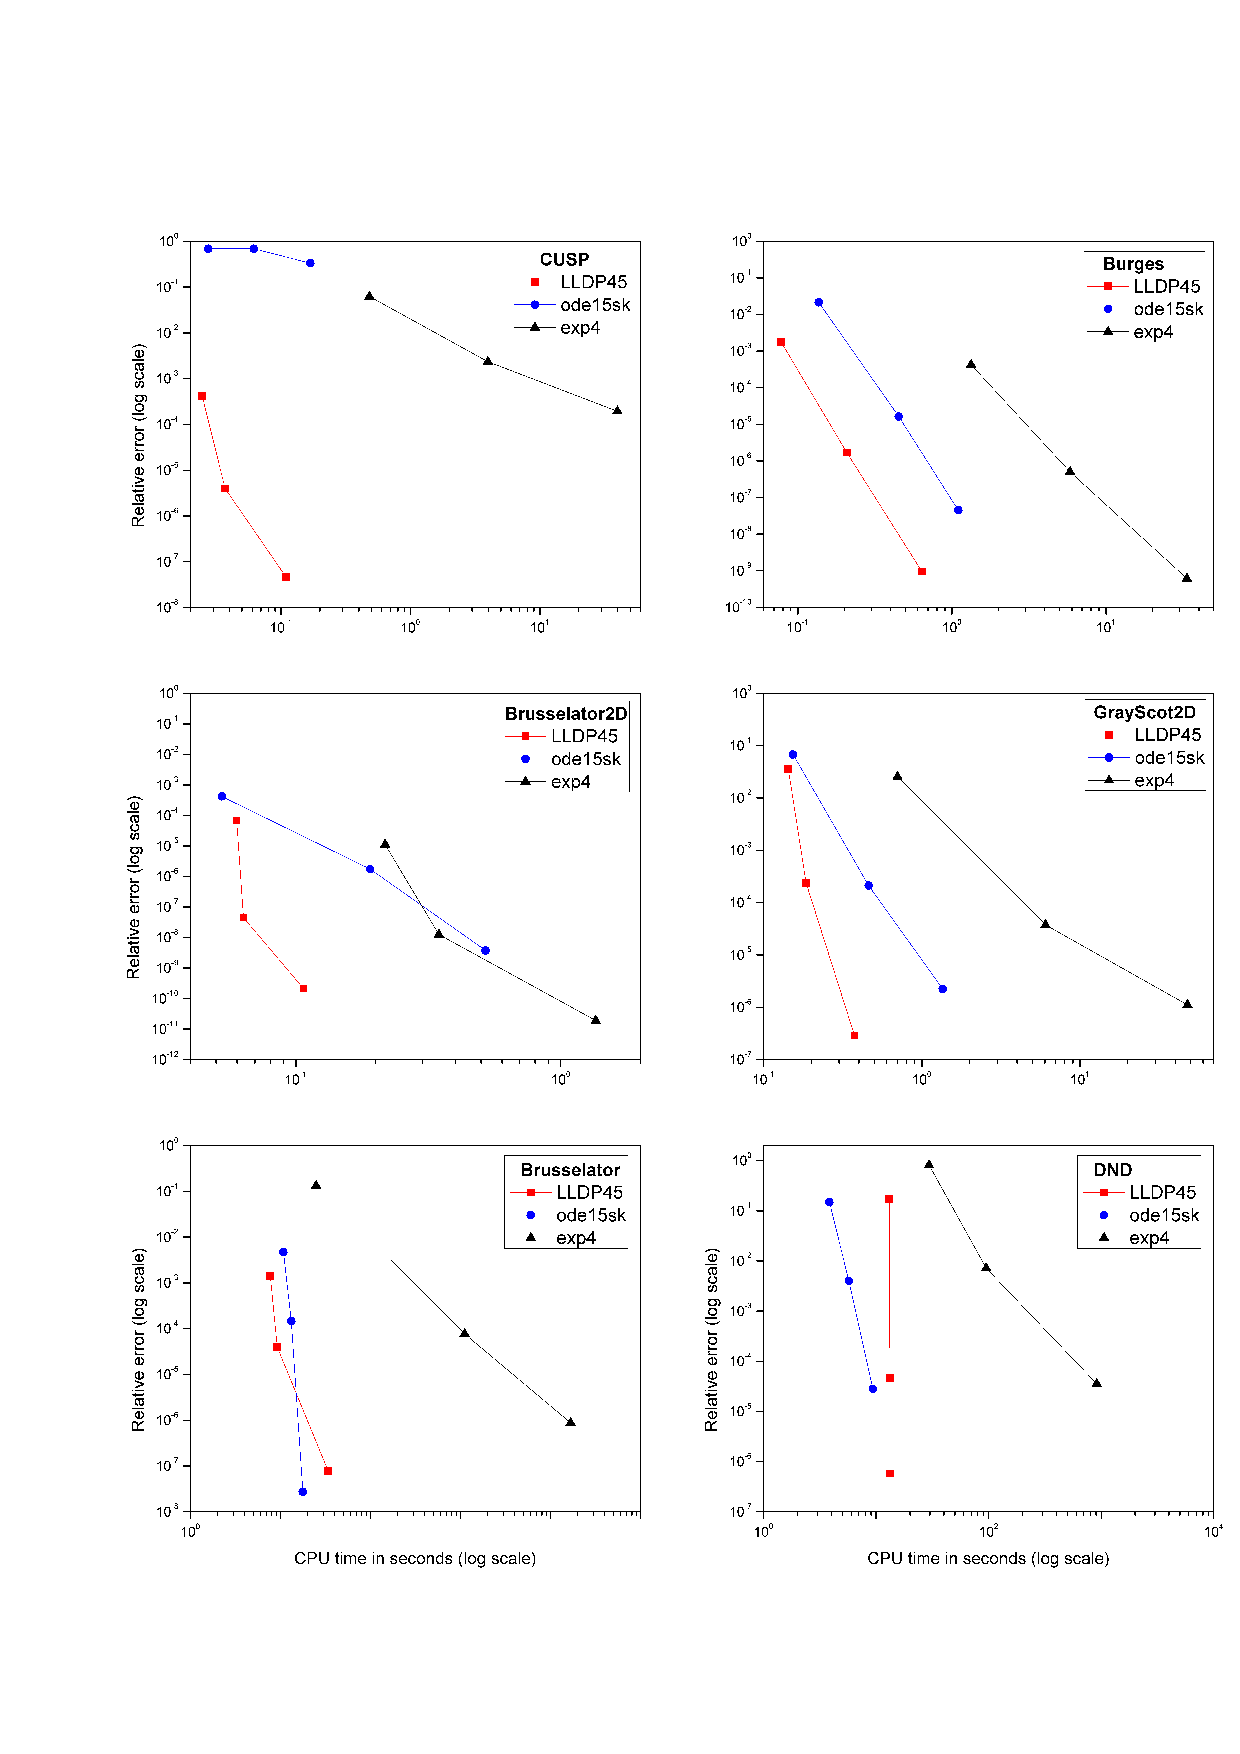
\includegraphics[scale=0.7]{Graphics/lldp/compare_graph.pdf}
	\vspace{-0.75in}
	\caption{ Diagrama log-log comparativo de precisión contra tiempo para cada uno de los códigos adaptativos en la integración de las seis ecuaciones de prueba. $\vartriangle$: código \emph{exp4}, $\circ$ : código \emph{ode15sk}, y $\square$: código \emph{LLDP45}}
	\label{num-exp-lldp-var-step:Fig1}
	\end{center}
\end{figure}

Para explicar estos resultados, para cada ecuación de prueba, los detalles de ejecución de cada código se presentan en una tabla. El error relativo \textit{RError} de cada código se mide nuevamente por la expresión (\ref{num-exp-lldp-fix-step:ER}) y el tiempo computacional relativo \textit{RTime} de cada código se calcula con respecto al tiempo computacional del código \emph{ode15sk}. Además, las tablas presentan el número de pasos \textit{A-Steps} aceptados y \textit{R-Steps} rechazados, así como el número de evaluaciones del campo vectorial \textit{f-Eval} y del Jacobiano \textit{J-Eval}. La dimensión mínima $\mf_ {min}$, máxima $\mf_ {max}$ y total $\mf_{total}$ de los subespacios de Krylov requeridos por los códigos \emph{LLDP45} y \emph{exp4} para integrar las ecuaciones de prueba sobre todo el intervalo de integración  también se dan, así como el orden de Padé mínimo $\pf_{min}$ y máximo $\pf_{max}$ requerido por el código \emph{LLDP45}. Para el código \emph{ode15sk}, $\mf_{min}$, $\mf_{max}$ y $\mf_{total}$ representan el número mínimo, máximo y total de iteraciones realizadas por el método GMRES sobre el intervalo de integración completo. Además, \textit{ME} denota el número de matrices exponenciales, \textit{ILU(0)} el número de factorizaciones LU incompletas, \textit{K-subspace} el número de aproximaciones del subespacio de Krylov, y \textit{GMRES} el número de sistemas lineales resueltos por el método GMRES. En las tablas, $d$ especifica el número de ecuaciones de cada ejemplo de prueba.

\begin{table}[htb]
	\caption{Desempeño de los códigos adaptativos \emph{exp4}, \emph{ode15sk} y \emph{LLDP45} en la integración de las ecuaciones  CUSP y Burgers.}
	\label{tab:num-exp-lldp-var-step:cuspburg}
	%\centering
	\begin{adjustbox}{width=0.8\columnwidth,center}
	\begin{tabular}{ ccccccccc }
		\hline
		& & \multicolumn{3}{c}{CUSP $M=500$, $d=1500$ } & & \multicolumn{3}{c}{Burgers $M=500$, $d=500$ }\\
		\cline{3-5} \cline{7-9}
		& Tolerancia & \emph{exp4} & \emph{ode15sk} & \emph{LLDP45} & & \emph{exp4} & \emph{ode15sk} & \emph{LLDP45} \\
		\hline
		& crudo & 17.5564 & 1.0000 & 0.8982 & & 9.7279 & 1.0000 & 0.5713 \\
		RTime  & medio & 64.1667 & 1.0000 & 0.6003 & & 12.9087 & 1.0000 & 0.4600 \\
		& refinado & 235.2210 & 1.0000 & 0.6489 & & 30.4093 & 1.0000 & 0.5799 \\
		\hline
		& crudo & 6.21e-02 & 6.89e-01 & 4.14e-04 & & 4.27e-04 & 2.14e-02 & 1.74e-03 \\
		RError  & medio & 2.35e-03 & 6.88e-01 & 3.97e-06 & & 4.98e-07 & 1.62e-05 & 1.67e-06 \\
		& refinado & 1.94e-04 & 3.32e-01 & 4.64e-08 & & 6.10e-10 & 4.49e-08 & 9.49e-10  \\
		\hline
		& crudo & 96 & 23 & 15 & & 175 & 245 & 77 \\
		A-Steps  & medio & 910 & 71 & 19 & &  963 & 809 & 291 \\
		& refinado & 9094 & 188 & 61  & & 5379 & 2593 & 1167 \\
		\hline
		& crudo & 1 & 0 & 0  & & 2 & 11 & 11 \\
		R-Steps  & medio & 0 & 3 & 1  & & 1 & 10 & 2 \\
		& refinado & 2 & 5 & 1  & & 1 & 11 & 0 \\
		\hline
		& crudo & 385 & 38 & 91  & & 708 & 520 & 529 \\
		$f$-Eval  & medio & 3642 & 101 & 121  & & 3857 & 1578 & 1759 \\
		& refinado & 36376 & 249 & 373  & & 21521 & 3021 & 7003 \\
		\hline
		& crudo & 95 & 1 & 4 &  & 175 & 2 & 72 \\
		$J$-Eval  & medio & 910 & 1 & 7 & &  963 & 1 & 123 \\
		& refinado & 9090 & 1 & 18 & &  5379 & 1 & 145 \\
		\hline
		& crudo & 291 & 0 & 15  & & 531 & 0 & 88 \\
		K-subspace  & medio & 2730 & 0 & 20  & & 2892 & 0 & 293 \\
		& refinado & 27288 & 0 & 62  & & 16140 & 0 & 1167 \\
		\hline
		& crudo & 0 & 36 & 0 &  & 0 & 518 & 0 \\
		GMRES  & medio & 0 & 99 & 0 &  & 0 & 1576 & 0 \\
		& refinado & 0 & 247 & 0 & &  0 & 3019 & 0 \\
		\hline
		& crudo & 293 & 0 & 15  & & 1422 & 0 & 165 \\
		ME  & medio & 2800 & 0 & 31 &  & 7724 & 0 & 491 \\
		& refinado & 27971 & 0 & 90  & & 43067 & 0 & 1352 \\
		\hline
		& crudo & 0 & 7 & 0  & & 0 & 44 & 0 \\
		ILU(0)  & medio & 0 & 16 & 0  & & 0 & 68 & 0 \\
		& refinado & 0 & 28 & 0  & & 0 & 106 & 0  \\
		\hline
		& crudo & 580 & 36 & 60  & & 2136 & 518 & 606 \\
		$\mf_{total}$  & medio & 5530 & 105 & 100 &  & 11588 & 1576 & 1529 \\
		& refinado & 55258 & 360 & 286  & & 64597 & 3019 & 4945 \\
		\hline
		& crudo & 2 & 1 & 4  & & 2 & 1 & 4 \\
		$\mf_{min}$  & medio & 2 & 1 & 4  & & 2 & 1 & 4 \\
		& refinado & 2 & 1 & 4 & &  2 & 1 & 4 \\
		\hline
		& crudo & 3 & 1 & 4 & &  11 & 1 & 26 \\
		$\mf_{max}$  & medio & 3 & 2 & 8  & & 8 & 1 & 10  \\
		& refinado & 4 & 2 & 8  & & 8 & 1 & 8 \\
		\hline
		& crudo & 0 & 0 & 3  & & 0 & 0 & 3 \\
		$\pf_{min}$  & medio & 0 & 0 & 3  & & 0 & 0 & 3 \\
		& refinado & 0 & 0 & 3  & & 0 & 0 & 3 \\
		\hline
		& crudo & 0 & 0 & 3 &  & 0 & 0 & 3 \\
		$\pf_{max}$  & medio & 0 & 0 & 3  & & 0 & 0 & 3  \\
		& refinado & 0 & 0 & 3 &  & 0 & 0 & 3 \\
		\hline
	\end{tabular}
	\end{adjustbox}
\end{table}


\begin{table}[htb]
	%\centering
	\caption{Desempeño de los códigos adaptativos  \emph{exp4}, \emph{ode15sk} y \emph{LLDP45} en la integración de las ecuaciones Brusselator2D y GrayScott2D .}	\label{tab:num-exp-lldp-var-step:bruss2dgray2d}
	\begin{adjustbox}{width=0.8\columnwidth,center}
	\begin{tabular}{  ccccccccc }
		\hline
		& & \multicolumn{3}{c}{Brusselator2D $M=50$, $d=5000$ } & & \multicolumn{3}{c}{GrayScott2D $M=50$, $d=5000$ }\\
		\cline{3-5} \cline{7-9}
		& Tolerancia & \emph{exp4} & \emph{ode15sk} & \emph{LLDP45} & & \emph{exp4} & \emph{ode15sk} & \emph{LLDP45} \\
		\hline
		& crudo & 4.1312 & 1.0000 & 1.1369 &  & 4.5759 & 1.0000 & 0.9329 \\
		RTime  & medio & 1.8186 & 1.0000 & 0.3325 &  & 13.1155 & 1.0000 & 0.4019 \\
		& refinado & 2.6035 & 1.0000 & 0.2055  & & 35.2552 & 1.0000 & 0.2771 \\
		\hline
		& crudo & 1.11e-05 & 4.18e-04 & 6.80e-05 & &  2.58e-02 & 6.75e-02 & 3.61e-02 \\
		RError  & medio & 1.26e-08 & 1.73e-06 & 4.44e-08 & &  3.76e-05 & 2.11e-04 & 2.39e-04 \\
		& refinado & 1.91e-11 & 3.74e-09 & 2.12e-10 & &  1.11e-06 & 2.24e-06 & 2.89e-07 \\
		\hline
		& crudo & 10 & 20 & 13 &  & 57 & 51 & 28 \\
		A-Step  & medio & 18 & 59 & 14 & &  596 & 133 & 38 \\
		& refinado & 98 & 141 & 22 & &  6000 & 353 & 91 \\
		\hline
		& crudo & 0 & 0 & 0  & & 3 & 0 & 0 \\
		R-Steps  & medio & 1 & 0 & 0  & & 4 & 0 & 0 \\
		& refinado & 1 & 0 & 0  & & 3 & 3 & 0 \\
		\hline
		& crudo & 42 & 28 & 79  & & 239 & 65 & 175 \\
		$f$-Eval  & medio & 77 & 73 & 85  & & 2398 & 157 & 235 \\
		& refinado & 397 & 194 & 133  & & 24011 & 453 & 547 \\
		\hline
		& crudo & 10 & 1 & 12 & &  57 & 1 & 26 \\
		$J$-Eval  & medio & 18 & 1 & 13  & & 596 & 1 & 26 \\
		& refinado & 98 & 1 & 19 & &  6000 & 1 & 34 \\
		\hline
		& crudo & 30 & 0 & 13 &  & 180 & 0 & 28 \\
		K-subspace  & medio & 57 & 0 & 14 &  & 1800 & 0 & 38 \\
		& refinado & 297 & 0 & 22  & & 18003 & 0 & 91 \\
		\hline
		& crudo & 0 & 26 & 0  & & 0 & 63 & 0 \\
		GMRES  & medio & 0 & 71 & 0 & & 0 & 155 & 0 \\
		& refinado & 0 & 192 & 0 & & 0 & 451 & 0 \\
		\hline
		& crudo & 48 & 0 & 13 & &  301 & 0 & 53 \\
		ME  & medio & 186 & 0 & 20  & & 2406 & 0 & 70 \\
		& refinado & 850 & 0 & 39  & & 24022 & 0 & 177 \\
		\hline
		& crudo & 0 & 6 & 0 & &  0 & 12 & 0 \\
		ILU(0)  & medio & 0 & 12 & 0  & & 0 & 22 & 0 \\
		& refinado & 0 & 24 & 0 &  & 0 & 56 & 0 \\
		\hline
		& crudo & 83 & 44 & 52  & & 501 & 150 & 226 \\
		$\mf_{total}$  & medio & 275 & 160 & 71  & & 4208 & 479 & 317 \\
		& refinado & 1263 & 512 & 139 &  & 42033 & 1540 & 576 \\
		\hline
		& crudo & 2 & 1 & 4  & & 2 & 1 & 4 \\
		$\mf_{min}$  & medio & 3 & 1 & 4  & & 2 & 1 & 4 \\
		& refinado & 3 & 1 & 4  & & 2 & 1 & 4 \\
		\hline
		& crudo & 8 & 2 & 4  & & 6 & 4 & 16 \\
		$\mf_{max}$  & medio & 8 & 3 & 8  & & 11 & 5 & 15 \\
		& refinado & 8 & 4 & 7  & & 8 & 6 & 8 \\
		\hline
		& crudo & 0 & 0 & 3  & & 0 & 0 & 3 \\
		$\pf_{min}$  & medio & 0 & 0 & 3 &  & 0 & 0 & 3 \\
		& refinado & 0 & 0 & 3  & & 0 & 0 & 3 \\
		\hline
		& crudo & 0 & 0 & 3  & & 0 & 0 & 3 \\
		$\pf_{max}$  & medio & 0 & 0 & 3 &  & 0 & 0 & 3  \\
		& refinado & 0 & 0 & 3  & & 0 & 0 & 3 \\
		\hline
	\end{tabular}
\end{adjustbox}
\end{table}



\begin{table}[htb]
	%\centering
	\caption{Desempeño de los códigos  adaptativos \emph{exp4}, \emph{ode15sk} y \emph{LLDP45} en la integración de las ecuaciones Brusselator y DND.}
	\begin{adjustbox}{width=0.8\columnwidth,center}
	\begin{tabular}{  ccccccccc }
		\hline
		& & \multicolumn{3}{c}{Brusselator $M=500$, $d=1000$ } & & \multicolumn{3}{c}{DND $M=500$, $d=500$}\\
		\cline{3-5} \cline{7-9}
		& Tolerancia & \emph{exp4} & \emph{ode15sk} & \emph{LLDP45} & & \emph{exp4} & \emph{ode15sk} & \emph{LLDP45} \\
		\hline
		& crudo & 2.3013 & 1.0000 & 0.7131  & & 7.6714 & 1.0000 & 3.4038 \\
		RTime  & medio & 84.1038 & 1.0000 & 0.6988  & & 5.9656 & 1.0000 & 2.3140  \\
		& refinado & 942.6567 & 1.0000 & 1.9127  & & 35.0007 & 1.0000 & 1.4193 \\
		\hline
		& crudo & 1.33e-01 & 4.67e-03 & 1.42e-03  & & 8.17e-01 & 1.49e-01 & 1.71e-01 \\
		RError  & medio & 7.68e-05 & 1.46e-04 & 3.91e-05  & & 7.11e-03 & 3.98e-03 & 4.63e-05 \\
		& refinado & 8.73e-07 & 2.72e-08 & 7.66e-08  & & 3.57e-05 & 2.79e-05 & 5.81e-07 \\
		\hline
		& crudo & 5896 & 6151 & 5421 &  & 3546 & 4580 & 19170 \\
		A-Steps  & medio & 253547 & 6995 & 9336  & & 21641 & 7260 & 19192 \\
		& refinado & 2585918 & 9847 & 34346  & & 209088 & 14628 & 28798 \\
		\hline
		& crudo & 40 & 5623 & 180  & & 4 & 1166 & 3176 \\
		R-Steps  & medio & 5 & 4827 & 0  & & 4 & 619 & 2708 \\
		& refinado & 4 & 4629 & 0  & & 2 & 145 & 105 \\
		\hline
		& crudo & 23714 & 19746 & 33607  & & 14198 & 13048 & 134077 \\
		$f$-Eval  & medio & 1014205 & 20842 & 56017  & & 86578 & 20159 & 131401 \\
		& refinado & 10343686 & 24450 & 206077  & & 836360 & 32775 & 173419 \\
		\hline
		& crudo & 5898 & 1865 & 4002 &  & 3546 & 581 & 17037 \\
		$J$-Eval  & medio & 253547 & 1894 & 131 & &  21641 & 294 & 15864  \\
		& refinado & 2585918 & 2123 & 135  & & 209088 & 9 & 2047 \\
		\hline
		& crudo & 17808 & 0 & 6601  & & 10644 & 0 & 22346 \\
		K-subspace  & medio & 760656 & 0 & 9336  & & 64935 & 0 & 21900 \\
		& refinado & 7757766 & 0 & 34346  & &  627270 & 0 & 28903 \\
		\hline
		& crudo & 0 & 19744 & 0  & & 0 & 13046 & 0 \\
		GMRES  & medio & 0 & 20840 & 0  & & 0 & 20157 & 0 \\
		& refinado & 0 & 24448 & 0  & & 0 & 32773 & 0 \\
		\hline
		& crudo & 17990 & 0 & 5601  & & 47516 & 0 & 22364 \\
		ME  & medio & 760690 & 0 & 9336  & & 85071 & 0 & 25659 \\
		& refinado & 7757796 & 0 & 34346  & & 790370 & 0 & 32463 \\
		\hline
		& crudo & 0 & 7603 & 0  & & 0 & 2163 & 0 \\
		ILU(0)  & medio & 0 & 6573 & 0  & & 0 & 1632 & 0 \\
		& refinado & 0 & 6732 & 0 & &  0 & 709 & 0 \\
		\hline
		& crudo & 35807 & 22779 & 22750  & & 81634 & 13046 & 95055 \\
		$\mf_{total}$  & medio & 1521373 & 41927 & 37344  & & 150087 & 20157 & 100908 \\
		& refinado & 15515593 & 64496 & 137384 &  & 1417707 & 32773 & 121723 \\
		\hline
		& crudo & 2 & 1 & 4  & & 2 & 1 & 4 \\
		$\mf_{min}$  & medio & 2 & 1 & 4 &  & 2 & 1 & 4  \\
		& refinado & 2 & 1 & 4  & & 2 & 1 & 4 \\
		\hline
		& crudo & 20 & 2 & 6  & & 36 & 1 & 14  \\
		$\mf_{max}$  & medio & 15 & 3 & 4  & & 36 & 1 & 12  \\
		& refinado & 36 & 3 & 4  & & 36 & 1 & 11 \\
		\hline
		& crudo & 0 & 0 & 3  & & 0 & 0 & 3 \\
		$\pf_{min}$  & medio & 0 & 0 & 3  & & 0 & 0 & 3 \\
		& refinado & 0 & 0 & 3  & & 0 & 0 & 3 \\
		\hline
		& crudo & 0 & 0 & 3  & & 0 & 0 & 3 \\
		$\pf_{max}$  & medio & 0 & 0 & 3  & & 0 & 0 & 3 \\
		& refinado & 0 & 0 & 3  & & 0 & 0 & 3 \\
		\hline
	\end{tabular}
\end{adjustbox}
	\label{tab:num-exp-lldp-var-step:brussdnd}
\end{table}

Las Tablas \ref{tab:num-exp-lldp-var-step:cuspburg} - \ref{tab:num-exp-lldp-var-step:brussdnd} muestran que, cuando el número de iteraciones del Algoritmo de Arnoldi ($\mf_{total}$) para calcular las funciones phi por vectores es similar o menor que el número de iteraciones del algoritmo GMRES ($\mf_{total}$) para resolver ecuaciones lineales, el costo computacional del código \emph{LLDP45} es menor que el del código \emph{ode15sk}. Este es un resultado esperado ya que estos dos algoritmos son las principales fuentes de complejidad computacional en los integradores mencionados. Además, aunque el número de exponenciales matriciales (\textit{ME}) calculadas con el código \emph{LLDP45} es mayor que el número de factorizaciones LU incompletas (\textit{ILU(0)}) del código \emph{ode15sk}, el costo computacional general de los primeros es menor que el de los segundos. Esto es así porque la exponencial matricial se calcula para matrices de dimensión significativamente menor (entre $\mf_{min}$ y $\mf_{max}$) que la dimensión $d$ de las matrices para las que se realiza la factorización LU incompleta. Por otro lado, con la excepción de la ecuación DND, el código \emph{LLDP45} requiere menos pasos de integración (\textit{A-Steps} + \textit{R-Steps}) que el código \emph{ode15sk}, que hace que la diferencia entre el número de evaluaciones de campos vectoriales (\textit{f-Eval}) de estos dos códigos no sea tan grande.

Además, las Tablas \ref{tab:num-exp-lldp-var-step:cuspburg}-\ref{tab:num-exp-lldp-var-step:brussdnd} muestran que la precisión del código \emph{exp4} es más cercana a la del código \emph{LLDP45} que a la del código \emph{ode15sk}. Sin embargo, el costo computacional del código \emph{exp4} es mucho más alto que el de los otros dos códigos. Esto se debe principalmente a la gran cantidad de pasos de integración (\textit{A-Steps} + \textit{R-Steps}), de aproximaciones del subespacio de Krylov (\textit{K-subspace}) y de iteraciones ($\mf_ {total}$) requerido por el código \emph{exp4} para integrar las ecuaciones de prueba.

Finalmente es importante notar que, debido a la falta de precisión del código \emph{ode15sk} para integrar la ecuación CUSP, la solución ``exacta'' de esta ecuación en (\ref{num-exp-lldp-fix-step:ER}) se estima mediante la fórmula continua (\ref{continuousLLRK45}) del código \emph{LLDP45} con $RTol = 10^{-12}$, $ATol = 10^{-14}$, $\mf_{min} = \mf_{max} = 100$ y factor de seguridad $\gamma_J=\infty$ para la reutilización de la matriz Jacobiana en el Algoritmo \ref{alg:jaccontrol}.

\subsubsection{Conclusiones del Capítulo}
En este Capítulo se construyeron nuevas fórmulas embebidas de Dormand y Prince localmente linealizadas para problemas de valor inicial de dimensiones no pequeñas utilizando las aproximaciones Krylov-Padé
con evaluación de Jacobiano en el cálculo de los productos de función phi por vector. Se derivaron cotas para los errores y condiciones de orden simples. Se desarrollaron estrategias adaptativas para la reutilización del Jacobiano, la selección del tamaño de paso de integración, la dimensión de Krylov y el orden de Padé con las que se implementaron esquemas con tamaño de paso fijo y dimensión
de Krylov variable, y esquemas con tamaño de paso y dimensión de Krylov variable. Se comprobó la eficacia de esos nuevos esquemas en la integración de diferentes ecuaciones y se constató que presentan igual o mejor precisión que los esquemas con los que fueron comparados requiriendo, en la mayoría de los casos, un número menor de pasos de integración.

%	La Aproximación Lineal Local de Orden Superior para EDO consiste en dividir en intervalos de tiempo consecutivos la solución de la ecuación original en una parte lineal , que es solución de la ecuación linealizada localmente, más una parte no lineal, que es solución de la representación diferencial del residuo. Combinando la aproximación Krylov-Padé con evaluación de Jacobiano, para aproximar la parte lineal, con las fórmulas embebidas Runge-Kutta de Dormand y Prince, para aproximar la parte no lineal, se construyeron nuevas fórmulas embebidas de Dormand y Prince localmente linealizadas para problemas de valor inicial de dimensiones no pequeñas. Para estas nuevas fórmulas se derivaron cotas para los errores y condiciones de orden simples ya que las cotas dependen de la dimensión del subespacio de Krylov, del orden de Padé y del orden del esquema Runge-Kutta utilizado.
%	
%	Para estas formulas construidas se desarrollaron diversas estrategias. Como el costo computacional de evaluar el Jacobiano en cada paso de integración puede ser grande se desarrolló una estrategia para su reutilización, donde bajo un criterio de error se decide si es posible utilizar el Jacobiano de pasos anteriores o es necesario volver a evaluarlo. Basado en la estrategia de selección de la dimensión de Krylov y el orden de Padé propuesta en el Capítulo \ref{chapter:solve-non-smal-lineal-eq} se desarrolló una estrategia específica para este estas nuevas fórmulas embebidas. Además desarrolló una estrategia adaptativa para la selección del tamaño de paso de integración.
%	
%	Con la aplicación de estas estrategias a las nuevas fórmulas embebidas de Dormand y Prince localmente linealizadas se implementaron esquemas con tamaño de paso fijo y dimensión de Krylov variable, y esquemas con tamaño de paso y dimensión de Krylov variable. Mediante la integración de diferentes ecuaciones  se comprobó la eficacia de esos nuevos esquemas y se constató que presentan igual o mejor precisión que los esquemas con los que fueron comparados requiriendo, en la mayoría de los casos, un número menor de pasos de integración.
